
\chapter{Massa, distanza, raggio e luminosit\'a. Fotometria, astrometria.}
\PartialToc

\section{Generalit\'a sull'astronomia sferica.}

\subsection{Sfera celeste}

\begin{figure}[!ht]
\centering
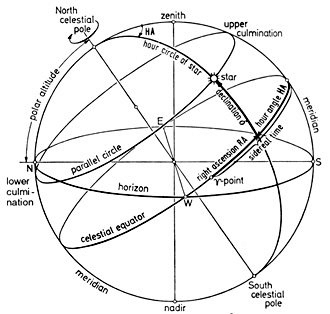
\includegraphics[width=(\textwidth),height=(\textheight-11mm),keepaspectratio]{CelestialSphere}
\caption{Sfera celeste.}
\end{figure}

\subsection{Declinazione e ascensione retta}



\clearpage


\subsection{Radio resonance in atomic and nuclear system.}

\subsection{Phase of the Earth respect distant stars}

Intersection of equatorial plane of the ecliptic at fixed epoch: $\gamma$-point. Instead of the angle $\phi$ one often uses the Universal Time
\begin{equation*}
UT1(t)=\frac{\phi(t)}{\omega_0}
\end{equation*}

\subsection{Standard for length has been forgone. Definition of speed of light.}

Tradizionalmente l'unit\'a di lunghezza, centimetro, si definisce tramite misure interferometriche come multiplo della lunghezza d'onda $\lambda_0$ di  una linea ottica stabile. \'E possibile misurare la velocit\'a della luce misurando la frequenza $\frac{c}{\lambda_0}$ tuttavia si preferisce \underline{definire} la velocit\'a della luce, se $c=1$ le lunghezze son misurate in secondi luce. This is appropriate to space physics in which distances are usually measure with transit time of light or radio pulses, timed by atomic clocks, or by means of doppler effect. In both cases only time standard is used. Inoltre la teoria della relativit\'a ci dice che lo spazio e il tempo sono uniti geometricamente in uno stesso concetto.

Time and frequency can by transerred from one point to another by EM signals
\begin{align*}
\frac{\nu_2}{\nu_1}=\overbrace{\sqrt{\frac{1-(\frac{v_1}{c})^2}{1-(\frac{v_2}{c})^2}}}^{\text{\hspace*{0pt} Transversal Doppler effect}}\underbrace{\frac{1-\frac{\vec{v_2}\cdot\hat{k}}{c}}{1-\frac{\vec{v_1}\cdot\hat{k}}{c}}}_{\text{\hspace*{0pt} ordinary Doppler effect}}
\end{align*}

%\subsection{Misure di parallasse}

\section{Keplerian problem}

\subsection{Prima legge di Keplero}

Sotto l'azione di una forza attrattiva un corpo celeste si sposta nel campo di attrazione dell'altro corpo celeste secondo una sezione conica: cerchio, ellisse, parabola, iperbole

\begin{usefull}{Prima legge di Keplero: consequence of inverse law of gravity.}
The orbit of a planet is an ellipse with the Sun at one focus.

For general two-body problem where the mass of secondary is not neglected both orbits are ellipses with their foci at their common barycentre
\end{usefull}

\subsection{Seconda legge di Keplero}

\begin{align*}
&m\TDof{t}(x\TDy{t}{y}-y\TDy{t}{x})=xF_y-yF_x&\intu{segue da legge fondamentale della dinamica newtoniana,}\\
&\TDof{t}(x\TDy{t}{y}-y\TDy{t}{x})=0&\intu{considerazioni geometriche implicano $\frac{F_x}{F_y}=\frac{x}{y}$.}\\
&x=r\cos{\theta},\quad y=r\sin{\theta}\\
&r^2\TDy{t}{\theta}=const&\intu{le aree spazzate dal raggio vettore nell'unit\'a di tempo sono una costante.}
\end{align*}

\begin{usefull}{Seconda legge di Keplero: conservation of angular momentum.}
The line joining a planet and the Sun sweeps out equal areas in equal intervals of time.

\end{usefull}

\subsection{Terza legge di Keplero}


Uguagliando le accelerazioni del moto circolare di velocit\'a angolare $\omega=\frac{2\pi}{T}$, $\omega^2r=\frac{4\pi^2r}{T^2}$, e dell'attrazione gravitazionale $G\frac{M+m}{r^2}$ si ottiene
\begin{equation*}
\frac{r^3}{T^2(M+m)}=\frac{G}{4\pi^2}=const
\end{equation*}

Per due corpi di massa $m_1$ e $m_2$ con semiasse maggiore delle rispettive orbite $a_1$ e $a_2$ e periodo $T_1$ e $T_2$
\begin{align*}
&\frac{a_1^3}{T_1^2(M_1+m_1)}=\frac{G}{4\pi^2}\\
&\frac{a_2^3}{T_2^2(M_2+m_2)}=\frac{G}{4\pi^2}\\
&\frac{T_1^2(M_1+m_1)}{T_2^2(M_2+m_2)}=\frac{a_1^3}{a_2^3}\\
&\frac{T_1^2}{T_2^2}=\frac{a_1^3}{a_2^3}&\intu{terza legge di Keplero ($M_1=M_2$, $m_1\approx m_2=0$).}
\end{align*}

\begin{usefull}{Terza legge di Keplero: inverse law of gravity}
The squares of the orbital periods of the planets are proportional to cubes of their semi-major axis.
\end{usefull}


\subsection{Orbite relative}

For general two-body problem where the mass of secondary is not neglected both orbits are ellipses with their foci at their common barycentre. La terza legge si riscrive
\begin{equation*}
P^2=\frac{4\pi^2}{GM}a^3
\end{equation*}

Il moto del pianeta relativo alla stella invece che al baricentro pu\'o essere trovato applicando un'accelerazione al sistema che cancella quella della stella (\mblock{\frac{Gm_p}{r^2}}), quindi la terza legge si riscrive

\begin{equation*}
P^2=\frac{4\pi^2}{G(M_*+M_p)}a_{rel}^3
\end{equation*}


Fatti:
\begin{itemize}
\item The measurements of relative separation doesn't arise for exoplanet orbit when the planet is unseen.

\item For binary star where an orbit is measured as a separtion and position angle of one star with respect another, the the combined system mass can be determined if $P$ and $a_{rel}$ are measurable. Individual masses can only be determined if mass ration can be established: from ratio of distances from barycentre or ratio of their speed around it.

\end{itemize}

For $m_p\ll M_*$ (in units of Earth's orbit of \SI{1}{\astronomicalunit})

\begin{equation*}
P\approx\SI{1}{\year}(\frac{a_{rel}}{\si{\astronomicalunit}})\expy{\frac{3}{2}}(\frac{M_*}{\msun{}})\expy{-\frac{1}{2}}
\end{equation*}

\subsection{Absolute orbits}

The orbit of the star around system star-planet barycentre is given by
\begin{align*}
&P^2=\frac{4\pi^2}{GM'}A_*^3\\
&M'=\frac{m_p^3}{(M_*+m_p)^2}&\intu{$a_*$ is the semi-major axis of stellar orbit around system barycentre}\\
&a_*:a_p:a_{rel}=m_p:M_*:(M_*+m_p)\\
&a_{rel}=a_*+a_p\\
&e_{rel}=e_*=e_p,\ P_{rel}=P_*=P_p\\
\end{align*}

Stellar position vs time allows maximum and minimum angular rate to be detrmined and hence positions of line of apsides: with orientation of orbit so determined appeal's to Kepler second law fixes orbit inclination.

Radial velocity measurement of host star gives informations on its barycentric orbital motion.

\section{Orbit specification}

A keplerian orbit in 3D is described by $a$, $e$ which specify the size and shape of elliptical orbit and $P$ related to $a$ and component masses through Kepler law, $t_p$ which is the position of the planet along its orbitat a particular reference time, and the three angle \mblock{(i,\Omega,\omega)} which represent the projection of true orbit into observed apparent orbit.



\tpc{!ht}{

\node at (0,0) {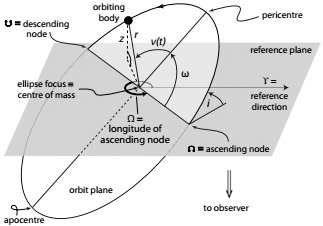
\includegraphics[width=(0.9\textwidth),height=(\textheight),keepaspectratio]{3Dorbit}};

\node at (0,-5) {\parbox{0.9\textwidth}{The reference plane is tangential to celestial sphere, i is the inclination of orbit plane. The true anomaly $\nu(t)$ is the time-dependent angle characterizing the object position along the orbit.}};
}
{(0,-6)}{6cm}{Elliptical orbit in 3D.}

\section{Luminosity function} 

\subsection{Trigonometric parallax}

Stars near the sun: object with total proper motion $\mu>\mu_0$

\subsection{spectroscopic parallax}

To apply this method, one must measure the apparent magnitude of the star and know the spectral type of the star. If the star lies on the main sequence, the spectral type of the star provides a good estimate of the star's absolute magnitude. Knowing the apparent magnitude (m) and absolute magnitude (M) of the star, one can calculate the distance (d, in parsecs) of the star using
\begin{align*}
&M − m = − 5\log{\frac{d}{10}}    
\end{align*}
The true distance to the star may be different than the one calculated due to interstellar extinction.

The spectroscopic absolute magnitude $M$ are derived from the intensity ratio of a number of Fraunhofer lines: the spectroscopic parallax are found using
\begin{equation*}
M=m+5+5\log{\pi_s}-a(\pi_s)
\end{equation*}

\subsection{Comparison of distribution of proper motion components and tangential}



\section{Indicatori di distanza.}

\subsection{Parallasse}

Le coordinate dei corpi celesti osservati dalla superficie terrestre sono topocentriche: la differenza tra diversi punti di osservazione sulla superficie terrestre non \'e trascurabile solo per i corpi del sistema solare e per stelle inferiori a \ang{;;0,00004} essa praticamente non esiste.

Fra le moltitudini di direzioni in cui l'astro \'e visibile dalla superficie quella principale \'e quella con origine nel centro della terra: fornisce la posizione geocentrica dell'astro e determina le sue coordinate geocentriche. L'angolo tra le direzioni secondo cui l'astro $M'$ sarebbe visibile da un qualsiasi punto sulla superficie e dal centro della Terra si chiama parallasse diurna: \'e l'angolo $p'$ sotto il quale dall'astro si vede il raggio della terra per il luogo di osservazione. La parallasse di un astro allo zenit nell'istante di osservazione \'e nulla, se l'astro \'e osservato all'orizzonte la sua parallasse diurna \'e massima ed \'e allora detta parallasse orizzontale $p$.


\subfile{tikz/diurnalparallax.tex}


La relazione fra i lati e gli angoli dei triangoli $TOM'$ e $TOM$ d\'a
\begin{align*}
&\frac{R}{\Delta}=\frac{\sin{p'}}{\sin{z'}},\quad \frac{R}{\Delta}=\sin{p}\\
&\sin{p'}=\sin{p}\sin{z'}
\end{align*}
 La parallasse orizzontale di tutti i corpi del sistema solare \'e molto piccola: Luna $p=\ang{;57;}$, Sole $p=\ang{;;8.79}$, per i pianeti \'e inferiore ad un primo.

I seni delle parallassi possono essere sostituiti con gli angoli stessi: $p'=p\sin{z'}$. 

Poich\'e la forma della Terra \'e quella di uno sferoide si definisce come raggio standard il raggio equatoriale $R_0=6379\si{\kilo\meter}$ e le parallassi orizzontali calcolate per questo raggio si chiamano parallassi orizzontali equatoriali $p_0$.


\subsection{Parallasse.}

Si misura lo spostamento della stella rispetto ad un riferimento di stelle fisse: parallasse diurna $\Delta T=1 \si{\hour}$ (sistema solare), parallasse annua $\Delta T$ di 6 mesi.


\begin{equation*}
    \pi_d=\frac{O_1O_2}{r}=\frac{2r_T\cos{\phi}}{r}
\end{equation*}
cio\'e l'angolo sotteso dalla distanza tra i due punti di osservazione visto dalla stella.

\begin{definition}{Parsec}
Distanza alla quale il semi-asse maggiore dell'orbita terrestre sottende:

\SI{1}{\arcsec}.

\end{definition}

Fatti:
\begin{itemize}
    \item Le stelle pi\'u vicine sono distanti qulache parsec.
    \item Potere risolutivo di un telescopio: $\frac{D}{\lambda}$. Per D=\SI{1}{\meter} e $\lambda=\SI{5000}{\angstrom}$ ho un potere risolutivo di \SI{0.1}{\arcsec}.
    \item Thecniche di best-fit: Numerose osservazioni vs ellissi teorica.
    \item Le osservazioni terrestri sono limitate dal seeing.
\end{itemize}

\subsubsection{Distanze corpi celesti.}

Conoscendo la parallasse equatoriale orizzontale $p_0$ dell'astro si calcola la sua distanza dal centro della terra
\begin{align*}
&\Delta=\frac{R_0}{\sin{p_0}}\\
&\sin{p_0}=p_0''\sin{\ang{;;1}}=\frac{p_0''}{\ang{;;206265}}\\
&\Delta=\frac{\ang{;;206265}R_0}{p_0''}&\intertext{$\uparrow$ le parallassi sono molto piccole: fornisce le distanze dei membri del sistema solare.}
\end{align*}
La distanza del corpo celeste \'e ottenuta nelle stesse unit\'a del raggio  della terra $R_0$.


\subsubsection{Parallasse annua.}

L'angolo sotto cui da una stella si vedrebbe il raggio medio dell'orbita terrestre nella condizione che la direzione verso questa stella sia perpendicolare a questo raggio si chiama parallasse annua $\pi$.

\begin{align*}
&\Delta=\frac{a}{\sin{\pi}}&\intertext{a \'e il raggio medio dell'orbita terrestre. Le parallassi delle stelle sono inferiori a \ang{;;1}:}\\
&\Delta=\frac{\ang{;;206265}a}{\pi''}
\end{align*}

Le parallassi determinate in base allo spostamento parallattico dell'astro sono dette trigonometriche. Le parallasi sono misurate con sufficiente precisione se la loro distanza non supera i 100\si{\parsec} ($\pi=\ang{;;0.01}$): si conoscono le parallassi di circa 6000 stelle vicino al sole.

\subsection{Moto proprio}

Spostamento progressivo rispetto ad un sistema stelle fisse (Blinking): proper motion is the astronomical measure of the observed changes in apparent positions of stars in the sky as seen from the center of mass of the Solar System compared to the imaginary fixed background of the more distant stars.

 This transverse sky motion is separate from the radial velocity, being the velocity moving toward or away from the observer in kilometres per second ($km/s$), as obtained from the Doppler shifts in starlight seen with a spectroscope. Knowledge of the proper motion, distance, and radial velocity allow approximate calculations of a star's true motion in space in respect to the Sun.

Stima distanza:
il moto proprio \'e inversamente proporzionale alla distanza, si deve ipotizzare la conoscenza della velocit\'a relativa rispetto al Sole V. Ipotizzando V costante per stelle vicine e uguale alla velocit\'a del Sole nell'ambiente locale trovo una relazione tra moto proprio sulla sfera celeste u, parallasse e velocit\'a sulla sfera celeste $V_0\sin{\lambda}$ con $\lambda$ angolo tra congiungente stella Sole e direzione del moto del Sole.

\begin{align*}
    &u=\frac{V_0\sin{\lambda}}{4.74}\pi&\intertext{$V_0$ in \si{\kilo\meter\per\second}}\\
    &H=\frac{\pi V_0}{4.74}&\intu{Parallasse secolare}
\end{align*}

Fatti:
\begin{itemize}
    \item Stelle vicine.
    \item Moto proprio progressivo.
    \item Ipotesi V costante applicabile a gruppo di stelle. Parallasse media: 
    \begin{equation*}
        \pi_{media}=\frac{4.74\sum u_i}{V_0\exv{\sin{\lambda}}N}
    \end{equation*}
\end{itemize}

\subsection{Parallasse di gruppo}

Associazione fisica di stelle con stessa velocit\'a relativa rispetto al sole
\begin{equation*}
    V=V_r\hat{r}+V_T\hat{e_T}
\end{equation*}
$V_T$ \'e osservabile mediante effetto Doppler, $V_T$ \'e legata al moto proprio. La parallasse di gruppo \'e 
\begin{equation*}
    \pi_{Gruppo}=\frac{4.74u}{V_R\tan{\lambda}}
\end{equation*}

\subsection{Parallasse statistica}

Ammassi considerati come gas di stelle caratterizzati da distribuzione di velocit\'a isotropa.

\subsubsection{Errore sulla magnitudine assoluta}

\begin{equation*}
    \Delta M_V=2\frac{\Delta\pi}{\pi}
\end{equation*}

\subsection{Unit\'a di misura distanza in astronomia}

\begin{itemize*}
\item Unit\'a astronomica, \si{\astronomicalunit}: Distanza media della Terra dal Sole.
\item \si{\parsec}: distanza corrispondente a una parallase annua di \ang{;;1}.
1\si{\parsec}=\num{30,86e12}\si{\kilo\meter}=\num{206265}\si{\astronomicalunit}=\num{3.26}\si{\lightyear}.
\item anno luce \si{\lightyear}: distanze percorsa in 1 anno dalla luce che viaggia a \num{300000}\si{\kilo\meter\per\second}.
1\si{\lightyear}=\num{9.460e12}\si{\kilo\meter}=\num{63240}\si{\astronomicalunit}=\num{0.3067}\si{\parsec}.
\end{itemize*}

Le distanze nel sistema solare sono espresse in unit\'a astronomiche: mercurio \'e a \num{0.387}\si{\astronomicalunit} dal Sole e Plutone a \num{39,44}\si{\astronomicalunit}.

Le distanze degli astri che si trovano al di fuori del sistema solare sono espresse in \si{\parsec}, \si{\kilo\parsec}, \si{\mega\parsec} ed anche anni luce:
\begin{align*}
&\Delta=\frac{1}{\pi\si{\arcsec}}\si{\parsec}\\
&\Delta=\frac{3.26}{\pi\si{\arcsec}}\si{\lightyear}
\end{align*}

\subsection{Unit\'a astronomica: parallasse del Sole.}

La determinazione diretta della parallasse del sole fornisce risultati grossolani.

Metodo indiretto: parallasse orizzontale di un pianeta che si avvicina alla terra ad una distanza inferiore di quella terra-sole, durante il XX secolo si usava Marte durante le sue opposizioni perieliche (\num{55e6}\si{\kilo\meter}). Supponiamo per semplicit\'a che al momento dell'opposizione perielica il Sole la Terra e Marte siano allineati:

la distanza terra-sole \'e $a_{\odot}=\si{\astronomicalunit}$ e Marte-Sole al perielio \'e $q=a(1-e)$ dove a \'e il semiasse maggiore ed e l'eccentricit\'a dell'orbita marziana, denotiamo con $\parallaxsun$ la parallasse orizontale equatoriale del sole, con $p$ la parallasse orizzontale equatoriale di Marte, con $\Delta$ lasua distanza geocentrica e con $R_0$ il raggio equatoriale della Terra.

\subfile{tikz/sunparallaxM.tex}

\begin{align*}
&R_0=a_0\sin{\parallaxsun}\\
&R_0=\Delta\sin{p}=(q-a_0)\sin{p}\\
&=[a(1-e)-a_0]\sin{p}\\
&a_0\parallaxsun=[a(1-e)-a_0]p&\intu{piccoli angoli, quindi:}\\
&\parallaxsun=[\frac{a}{a_0}(1-e)-1]p&\intu{Il rapporto $\frac{a}{a_0}$ viene calcolato applicando la terza legge di Keplero, mentre la parallasse di Marte p e la sua eccentricit\'a e sono determinate osservativamente.}
\end{align*}

A partire dal 1970:
\begin{equation*}
\parallaxsun=\ang{;;8.794},\quad 1\si{\astronomicalunit}=\num{149.6e6}\si{\kilo\meter}
\end{equation*}

\subsection{Metodi dinamici e fisici}
I metodi dinamici determinano la distanza attraverso la legge di gravitazione universale, i metodi fisici sfruttano la propagazione delle onde radio ($\Delta=\frac{ct}{2}$).


\section{Massa e raggio.}

\subsection{Sole}

La massa la determino usando il moto orbitale della Terra
\begin{align*}
    &\frac{G\msun{}}{d_{T\odot}^2}=\frac{v_T^2}{d_{T\odot}}\\
    &d_{T\odot}=\SI{1}{\astronomicalunit}=\SI{1.496e13}{\cm}\\
    &v_T=\SI{2.978e6}{\cm\per\second}&\intertext{da cui la massa del Sole:}\\
    &\msun{}=\frac{v_T^2d_{T\odot}}{G}=\SI{1.99e33}{\gram}
\end{align*}

e il raggio

\begin{align*}
    &\text{Raggio apparente}=\ang{;15;59.63}\\
    &\rsun{}=\SI{6.96e10}{\cm}
\end{align*}

\subsection{Determinazione della massa}



 \begin{itemize*}
 \item Misurando la gravit\'a alla superficie del corpo considerato.
 
\begin{align*}
g=G\frac{m}{R^2}&\intu{accelerazione di gravit\'a sulla superficie terrestre:}\\
m=\frac{gR^2}{G}
\end{align*}
 
\item Applicando la terza legge di Keplero.

Permette di determinare il rapporto tra la massa del Sole e la massa di un pianeta se questo possiede almeno un satellite e si conosce la distanza satellite-pianeta e il periodo del satellite attorno al pianeta:

\begin{align*}
&\frac{T^2(M+m)}{t_S^2(m+m_S)}=\frac{a^3}{a_S^3}\\
&(\frac{M}{m}+1):(1+\frac{m_S}{m})=\frac{t_S^2a^3}{T^2a_S^3}&\intertext{Il rapporto $\frac{M}{m}$ \'e grande per tutti i pianeti, il rapporto $\frac{m_S}{m}$ \'e piccolo ma in per il sistema Terra-Luna non trascurabile (per i satelliti di Giove si).}
\end{align*}

\item Analizzando le perturbazioni provocate da un astro sui moti di altri corpi celesti.

Le masse dei pianeti senza satelliti sono determinate mediante le perturbazioni create al moto di altri corpi.

\item Red-Shift radiazione.

\end{itemize*}
 

\subsection{Interferometro di Hanbury-brown: Dimensioni angolari.}


\section{Fotometria}
Luminosita' e colore di una stella. la magnitudine (varie definizioni). Sistemi fotometrici, indici di colore e temperatura efficace. 
%http://www.astro.sunysb.edu/fwalter/PHY515/photometry.html


\subsection{Flusso di radiazione osservato}

Sirus \'e 2 miliardi di volte pi\'u brillante della stella pi\'u debole osservata con i telescopi: gran parte della differenza di luminosit\'a apparente \'e dovuta al range di distanze. L'osservazione di ammassi di stelle mostra che $\num{e-6}\lsun{}\leq L\leq \num{e6}\lsun{}$.

\begin{definition}{Stellar photometry}
Tecniche per determinare la luminosit\'a e il colore stellare misurando un range largo dello spettro stellare
\end{definition}


\begin{definition}{Flusso monocromatico $F_{\lambda}$}
$F_{\lambda}$ \'e l'energia emessa dalla stella per unit\'a di tempo, per unit\'a di superficie alla lunghezza d'onda $\lambda$.
\end{definition}

Fatti:
\begin{itemize}
\item Le stelle rapidamente rotanti non hanno forma sferica e la luminosit\'a non \'e uniformemente distribuita sulla superficie
\item La luce riflessa dai pianeti (emissione termica: rilascio energia assorbita) \'e parzialmente anisotropa
\item La simmetria sferica non esiste per emissione non termica: emissione fotoni dovuta al moto di cariche in campo magnetico.
\end{itemize}

\begin{definition}{Luminosit\'a bolometrica.}
\begin{align*}
&L=\int_0^{\infty}L_{\lambda}\,d\lambda=4\pi R^2\int_0^{\infty}F_{\lambda}\\
&L=4\pi R^2\sigma T_e^4,\ \sigma=\num{5.67e-5}(cgs)
\end{align*}
\end{definition}

\begin{align*}
&f_{\lambda}=\frac{\lmono{}}{4\pi r^2}=\lmono{}(\frac{R}{r})^2,\ f=\frac{L}{4\pi r^2}=L(\frac{R}{r})^2&\intu{Flusso di radiazione raccolto da una superficie unitaria: radiazione/superficie * elemento superficie stellare diviso elemento superficie osservatore. Parte della radiazione viene assorbita dal mezzo interstellare e dall'atmosfera}\\
&f_{\lambda}'=A_{\lambda}f_{\lambda}&\intu{effetto assorbimento mezzo interstellare}\\
&f_{\lambda}''=D_{\lambda}(\theta)A_{\lambda}f_{\lambda}&\intu{effetto assorbimento mezzo interstellare e atmosfera}
\end{align*}

\subsubsection{Assorbimento mezzo interstellare}

Discovered in '20: were observed stars whose color temperature were much lower than the temperature indicated by degree of ionization in their spectra (since interstellar reddening follow law similar to temperature reddening). Interstellar reddening was discovered trough comparison of distance of galactic clusters obtained geometrically and photometrically.

Fatti:
\begin{itemize}
\item Is selective with respect to wavelength: increase of observed color index of about \SI{0.31}{\magnitude\per\kilo\parsec}.
\item Doesn't follow Rayleigh's law $I\propto\frac{1}{\lambda^4}$ but varies more nearly as $\frac{1}{\lambda}$.
\end{itemize}

\subsection{Sistemi fotometrici}


\begin{itemize}
    \item UBV: Blue filter is chosen to reduce balmer continuum on blue magnitude. The zero point of blue-yellow color index has been set at A0 
\end{itemize}


\begin{figure}[!ht]
\centering
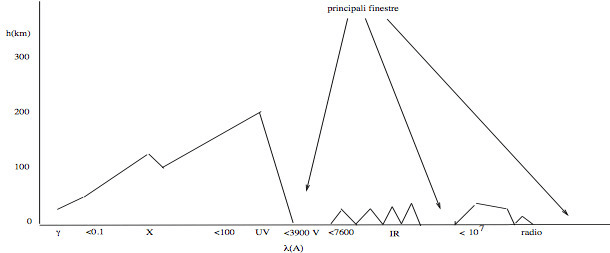
\includegraphics[width=(0.9\textwidth),height=(\textheight-11mm),keepaspectratio]{obswin}
\caption{Sopra la linea \'e possibile fare astronomia.}
\end{figure}

\begin{definition}{Luce visibile}
Visibile \numrange{3900}{7600}\si{\angstrom}
\end{definition}

\begin{definition}{Curve di sensibilit\'a del rivelatore $S(\lambda)$.}
\begin{itemize}
\item Curva visuale \numrange{5500}{6000}\si{\angstrom}
\item Curva fotografica \numrange{4000}{4500}\si{\angstrom}
\item Curva foto-visuale: riproduce il caso visuale tramite un filtro giallo e una lastra fotografica
\end{itemize}
\end{definition}

\begin{definition}{Larghezza banda (fotometria)}
\begin{itemize}
\item Banda larga: $>100\si{\angstrom}$.
\item Banda media: $\approx100\si{\angstrom}$.
\item Banda stretta: $<100\si{\angstrom}$
\end{itemize}
\end{definition}

\begin{figure}[!ht]
\centering
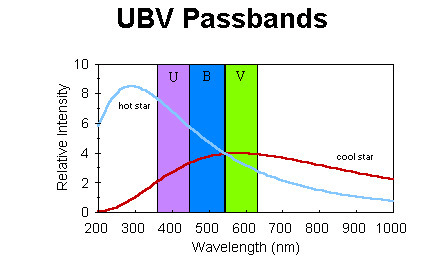
\includegraphics[width=(0.9\textwidth),height=(\textheight-11mm),keepaspectratio]{ubv}
\caption{Filtri passabanda UBV.}
\end{figure}

\clearpage



Sistemi che permettono osservazioni mediante filtri:
\begin{itemize}
\item Johnson-Morgan: (UBV) + 2 filtri VB (fotografici) e un terzo centrato sui \SI{3600}{\angstrom} in corrispondenza del salto di Balmer (FWHM:\SI{900}{\angstrom}, \SI{1000}{\angstrom}, \SI{700}{\angstrom}).
\item Ginevra: (UBV) + filtri nel visibile (a banda stretta)
\item Stromgren: 3 filtri UBV a banda stretta filtro Y intorno ai \SI{4700}{\angstrom} e un filtro centrato su linea idrogeno $H\beta$ ($2\to4$).
\item WUBV: band ($\lambda,\ \Delta\lambda$\si{\angstrom}) W($3270,\ 150$), U($3670,\ 260$), B($4295,\ 420$), V($5450,\ 850$)
\end{itemize}

Risposta di un Fotometro (visuale):
\begin{align*}
&f(\lambda)=S_VD_{\lambda}(\theta)A_{\lambda}f_{\lambda}\\
&I_V=\int_0^{\infty}f(\lambda)\,d\lambda\\
&=\int_0^{\infty}S_VD_{\lambda}(\theta)A_{\lambda}\lmono{}\frac{\,d\lambda}{4\pi r^2}
\end{align*}

Fatti:

\begin{itemize}
\item Wide band photometry: $B-V$. Limited by interstellar absorption.
\item Narrow band photometry: Strenght $H\gamma,\ H\delta$ to luminosity.
\item Ultraviolet method: Barbier-Chalonge, Balmer discontinuity at \mblock{\lambda=\SI{3647}{\angstrom}}.
\item Photographic method: ratio of absorption-line pairs.
\end{itemize}


\subsection{Magnitudine relativa}

In 1856, Norman Robert Pogson formalized the system by defining a first magnitude star as a star that is $100$ times as bright as a sixth-magnitude star, thereby establishing the logarithmic scale still in use today. This implies that a star of magnitude $m$ is $2.512$ times as bright as a star of magnitude $m+1$.

\subsubsection{Formula gi Pogson}

\begin{definition}{Magnitudine relativa}
\begin{equation*}
m_V=-2.5\log{I_V}+\const{}
\end{equation*}

Magnitudine di riferimento:
\begin{equation*}
-2.5\log{I_V*}+\const{}=0
\end{equation*}

\end{definition}

Vega ($\alpha$-Lyr)  ha magnitudine relative circa zero.

\subsection{Magnitudine assoluta}

Absolute magnitude is the measure of intrinsic brightness of a celestial object. It is the hypothetical apparent magnitude of an object at a standard distance of exactly \SI{10}{\parsec} (\SI{32.6}{\lightyear}) from the observer, assuming no astronomical extinction of starlight. This places the objects on a common basis and allows the true energy output of astronomical objects to be compared without the distortion introduced by distance. As with all astronomical magnitudes, the absolute magnitude can be specified for different wavelength intervals; for stars the most commonly quoted absolute magnitude is the absolute visual magnitude, which uses only the visual (V) band of the spectrum (UBV system). Also commonly used is the absolute bolometric magnitude, which is the total luminosity expressed in magnitude units that takes into account energy radiated at all wavelengths, whether visible or not.

\begin{definition}{Magnitudine assoluta}
\begin{equation*}
M_V=m_V+5\log{\frac{\SI{10}{\parsec}}{r}}-A
\end{equation*}
r \'e la distanza della stella (in pc), A rappresenta l'assorbimento interstellare (media di $\log{A_{\lambda}}$) dipende dalla distanza ed \'e massimo sul piano galattico ($\exv{A}\approx\frac{r}{2000\si{\parsec}}$).
\end{definition}

\begin{definition}{Magnitudine bolometrica.}
\'E la magnitudine che otterremmo raccogliendo tutta la luce che giunge all'orbita terrestre (\mblock{A_{\lambda}S_{\lambda}(\theta)=1}). Introduco la correzione bolometrica $BC$:
\begin{equation*}
m_{Bol}=m_V+BC
\end{equation*}
Scelgo che $BC\approx0$ per stelle che emettono nel visibile.
\end{definition}

Fatti:
\begin{itemize}
\item Allen (2000): $BC=0$ per supergiganti di classe di luminosit\'a 1 e tipo $F2$.
\end{itemize}

\begin{definition}{Magnitudine bolometrica assoluta.}
Magnitudine bolometrica assoluta:
\begin{align*}
&M_{Bol}=-2.5\log{\frac{L}{\lsun{}}}+4.74&\intertext{$4.74$ sarebbe la magnitudine bolometrica assoluta del sole se fosse a \SI{10}{\parsec}}\\
&(\lsun{}=\SI{3.845e33}{\erg\per\second})
\end{align*}
\end{definition}

\clearpage

\subsection{Indici di colore.}

\begin{definition}{Indicatori bande sistemi fotometrici}
Zona dello spettro: Lettera del filtro, Punto medio della radiazione effettiva  $\lambda_{eff}$
per il filtro standard, $FWHM$, Variante/i,	Descrizione.
\begin{itemize}

\item   Ultravioletto:
 U , $365 nm$ ,	$66 nm$ ,	$u, u', u*$,	"U" sta per "ultravioletto".
 
\item Visibile:

B, $445 nm$ , $94 nm$, $b$,	"B" sta per "blu".

V,	$551 nm$ , $88 nm$, $v, v'$, "V" sta per "visibile".

G, , , $g, g'$, "G" sta per "green" (verde).

R, $658 nm$, $138 nm$, $r, r', R', Rc, Re, Rj$, "R" sta per "rosso".

\item Infrarosso vicino:

I, $806 nm$, $149 nm$, $i, i', Ic, Ie, Ij$, "I" sta per "infrarosso".

Z ,,, z, z',.

Y $1020 nm$, $120 nm$, $y$,.

J, $1220 nm$, $213 nm$, $J', Js$,.

H, $1630 nm$, $307 nm$,,,.

K, $2190 nm$, $390 nm$, $K$, Continuum, K', Ks, Klong, K8, nbK.

L, $3450 nm$, $472 nm$, $L', nbL'$,.

\item Infrarosso medio:

M, $4750 nm$, $460 nm$, $M', nbM$,.	
N , , , $N1, N2, N3$,.

Q, , ,$ Q'$,.
 	
\end{itemize}     

\end{definition}

\begin{align*}
&U-B=m_U-m_B\\
&B-V=m_B-m_V&\intertext{Una stella blu ha $B-V$ pi\'u basso di una stella rossa.}
\end{align*}

Fissiamo le costanti per avere per stelle $A0$
\begin{equation*}
m_V\approx m_B\approx m_U
\end{equation*}
La distanza provoca uno spostamento verso il rosso: $E(B-V)\approx0.3 A$, $E(U-B)\approx0.1A$.

\subsection{SAAO Standards for Optical Photometry}

\begin{itemize}
    \item Harvard E-Region. 48 equal areas into which Pickering divided the sky
    \item $UBVR_cI_c$. optical UBV + R e I. The colour $(V-I)_C$ is a good temperature indicator that is less sensitive to gravity effects than $(B-V)$, $(U-B)$ is strongly affected by H Balmer absorption: together these 3 colors are usefull to determine color excess of stars (scattering/absorption of star light by interstellar dust).
    \item Str\"omgren $uvby$. Intermediate-band photometric system, narrower band. Metallicity index \mblock{m_1=(v-b)-(b-y)}. The index \mblock{c_1=(u-v)-(v-b)} is a mesure of Balmer discontinuity and thus a T index for OB stars and a surface gravity index for AF stars.
    \item $H\beta$. Intermediate pass-band (\mblock{FWHM\approx\SI{150}{\angstrom}}) and a narrow pass-band (\mblock{FWHM\approx\SI{30}{\angstrom}}) both centered on the Balmer $H\beta$ line of Hydrogen. A magnitude difference between the two filter measure the strength of $H\beta$: good surface gravity/luminosity index for OB stars and good T index for AF stars
    \item DDO. Intermediate pass-band filters (and narrow filter), $FWHM\approx\SI{80}{\angstrom}$. The system was intended for measure integrated light from galaxy nuclei to construct stellar population model for galaxies. The six pass-band are centered between \SIrange{3500}{4800}{\angstrom} and colours of the form $C(35-38)$, $C(38-41)$, \ldots are derived giving parameter related to Balmer discontinuity, line blanketing near \SI{4100}{\angstrom}, strength of CN absorption and G-band break. Usefull for F-K type stars.
\end{itemize}



\section{Stelle doppie.}

\begin{todo}{Stelle doppie}
Le stelle doppie: metodi di osservazione, problematiche generali; effetti di selezione. le stelle doppie per la stima delle masse e dei raggi delle stelle. relazioni massa-raggio e massa-luminosit\'a. 
\end{todo}


Circa la met\'a delle stelle osservate fanno parte di un sistem binario e in sistemi multipli si hanno spesso sottosistemi doppi poco influenzati dalle altre masse.

Dal moto orbitale posso ricavare in situazioni favorevoli
\begin{itemize}
    \item Somma delle masse
    \item Rapporto delle masse
    \item (Luminosit\'a delle componenti)
    \item Periodo orbitale
\end{itemize}


\subsection{Binarie visuali.}

Separazione angolare minore osservabile:

\SI{1}{\arcsec} dalla Terra, limitata dalle dimensioni del telescopio dallo spazio (circa \SI{e-2}{\arcsec}).

I sistemi pi\'u facilmente osservabili sono quelli a periodo lungo (grande separazione) e non troppo distanti:

un sistema a \SI{100}{\parsec} ha separazione \SI{1}{\arcsec} se \'e largo \SI{100}{\astronomicalunit} (per masse solari il periodo \'e di centinaia di anni).

Quindi le regole di selezione porteranno ad osservare con maggior frequenza sistemi vicini e di periodo lungo ma osservabile con stessa luminosit\'a delle componenti (sistemi gemelli).

Masse e raggi.

Terza legge di Keplero:
\begin{align*}
    &M_1+M_2=\frac{4\pi^2a^3}{GP^2}\\
    &M_1+M_2=\frac{1}{P^2}(\frac{a}{\Pi})^3&\intu{P in anni solari, a in arcsec, M's in $\msun{}$}
\end{align*}

quindi nota la parallasse $\Pi$, osservati $P$ e $a$ si ricava la somma delle masse.

Per ricavare le masse analizzo il moto delle due componenti rispetto al CM:

\subfile{tikz/binaryV}

\begin{equation*}
    \frac{M_1}{M_2}=\frac{a_2}{a_1}
\end{equation*}

\subsection{Binarie spettroscopiche.}

Misura la variazione periodi della velocit\'a radiale misurata tramite effetto Doppler.

Classi di oggetti privilegiati:
\begin{itemize}
    \item Oggetti non troppo deboli: spettro a media dispersione.
    \item Periodi non troppo lunghi: un periodo di $T\approx\SI{100}{\year}$ per masse solari comporta una $V_R\approx\SI{1}{\kilo\meter\per\second}$ (difficile da osservare), un periodo $T\approx\SI{1}{\year}$ comporta una $V_R\approx\SI{10}{\kilo\meter\per\second}$.
    \item A seconda del rapporto fra le luminosita sono osservabili una sola o entrambe le componenti.
\end{itemize}

Masse e raggi.
Sistema non risolto spazialmente, tengo conto dell'inclinazione del piano dell'orbita rispetto al piano notmale alla linea di vista moltiplicando ambo i membri della terza legge di Keplero per $\sin{i}$:

\begin{equation*}
    (M_1+M_2)\sin^3{i}=\frac{4\pi a^3\sin^3{i}}{GP^2}
\end{equation*}

Se sono note le velocit\'a radiali di ambo le componenti da \mblock{\frac{M_1}{M_2}=\frac{a_2\sin{i}}{a_1\sin{i}}=\frac{v_{2R}}{v_{1R}}} ottengo \mblock{M_1\sin^3{i}$ e $M_2\sin^3{i}}.

Se \'e nota solo una componente posso misurare
\begin{align*}
    &\frac{4\pi^2}{GP^2}a_1^3\sin^3{i}=(M_1+M_2)\sin^3{i}\frac{M_2^3}{(M_1+M_2)^3}&\intertext{quindi}\\
    &a=a_1+a_2=a_1(1+\frac{a_2}{a_1})=a_1(1+\frac{M_1}{M_2})\\
    &=a_1\frac{(M_2+M_1)}{M_2}
\end{align*}

Definisco la funzione di massa

\begin{equation*}
    f(M_1,M_2)=\frac{v_1^3P}{2\pi G}=\frac{(M_2\sin^3{i})^3}{(M_1+M_2)^2}
\end{equation*}

Fatti:
\begin{itemize}
    \item Se il sistema \'e anche fotometrico posso ricavare $\sin{i}$.
    \item Per $i=\frac{\pi}{2}$ ottengo un limite inferiore per le masse.
\end{itemize}

\subsection{Binarie a eclisse (fotometriche).}

Tecniche fotometriche: eclisse parziale/totale fra le componenti.

Osservabilit\'a dipende da inclinazione del piano dell'orbita rispetto alla linea di vista: l'angolo massimo dipende dalle dimensioni degli astri e dalla loro separazione.

Fatti:
\begin{itemize}
    \item Un periodo di un anno fra 2 stelle simili al Sole permette eclissi se l'angolo fra la linea di vista e il piano dell'orbita \'e minore di \ang{1;;}
    \item Separazione di pochi raggi stellari: per stelle non giganti periodo di giorni.
\end{itemize}

Masse e raggi.

\begin{figure}[!ht]
\centering
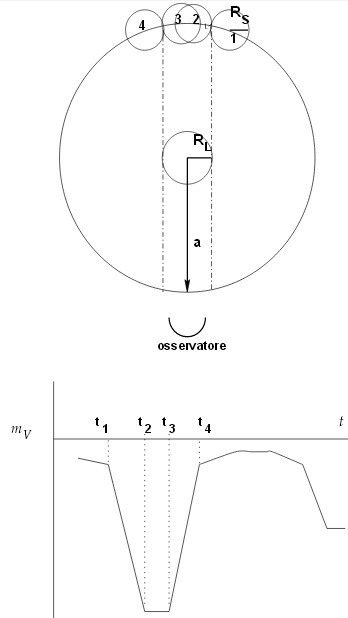
\includegraphics[width=\textwidth,height=0.9\textheight,keepaspectratio]{binaryE}
\caption{Binarie a eclisse.}\label{fig:binaryE}
\end{figure}

Analisi curva di luce (vedi \ref{fig:binaryE}):

\begin{align*}
    &M_1+M_2=\frac{4\pi^2a^2}{P^2G}&\intu{Terza legge di Keplero,}\\
    &\frac{t_4-t_1}{P}=\frac{2(R_L+R_S)}{2\pi a}\\
    &\frac{t_3-t_2}{P}=\frac{2(R_L-R_S)}{2\pi a}&\intertext{quindi ricavo $\frac{R_L}{a}$, $\frac{R_S}{a}$.}
\end{align*}

Ricavo le relazioni semi-empiriche per le stelle della MS \index{Relazioni semiempiriche MS.}:

\begin{align*}
    &R\propto M\expy{\frac{1}{2}}\\
    &L\propto \left\{\begin{array}{c}
         M^4,\ M<0.8\msun{}  \\
         M^3,\ M>0.8\msun{}  \\
    \end{array}\right.
\end{align*}

\clearpage


\chapter{Spettri stellari: Spettroscopia.}
\PartialToc

\section{Formazione spettri stellari: righe di assorbimento.}
Classificazione degli spettri stellari. Classi di luminosit\'a. 
Elementi di teoria delle righe spettrali. larghezza naturale di una riga. Introduzione ai fenomeni di allargamento. 
Allargamento delle righe spettrali: vari effetti. Spettri ad alta, media e bassa dispersione.

\subsection{Emission Line (Nebulae)}

Strong emission line owing to allowed/forbidden transitions of heavy elements (N, O, Ne, S, Cl, Ar, P, Fe, Ca, Mn, Cr, V, Co, Ni) in varous ionization stages: allowed transition are accounted for by electric dipole radiation, whereas forbidden transitions are due to magnetic dipole / electric quadrupole radiation. Forbidden emeission lines result from collisional excitation of metastable levels were first identified in gaseus nebula by Bowen (1928).


\subsubsection{Idrogeno}

\begin{definition}{Salto di Balmer}
Balmer jump or Balmer discontinuity is the difference of intensity of the stellar continuum spectrum on both sides of the limit of the Balmer series of hydrogen at \SI{364.6}{\nano\meter}. It is caused by electrons being completely ionized directly from the second energy level of a hydrogen atom (bound-free absorption), which creates a continuum absorption at wavelengths shorter than \SI{364.6}{\nano\meter}.

In some cases the Balmer discontinuity can show continuum emission, usually when the Balmer lines themselves are strongly in emission. Other hydrogen spectral series also show bound-free absorption and hence a continuum discontinuity, but the Balmer jump in the near UV has been the most observed.

The strength of the continuum absorption, and hence the size of the Balmer jump, depends on temperature and density in the region responsible for the absorption. At cooler stellar temperatures, the density most strongly affects the strength of the discontinuity and this can be used to classify stars on the basis of their surface gravity and hence luminosity. This effect is strongest in A class stars, but in hotter stars temperature has a much larger effect on the Balmer jump than surface gravity.
\end{definition}

\begin{definition}{Serie di Balmer}
\begin{figure}[!ht]
\centering
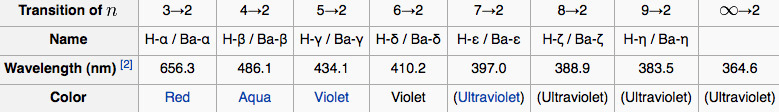
\includegraphics[width=(0.9\textwidth),height=(\textheight-11mm),keepaspectratio]{Bserie}
\caption{Serie di Balmer.}
\end{figure}
\end{definition}

\subsection{Atmosfera stellare}

Lo spettro di una stella \'e caratterizzato da una distribuzione simile a quella di un corpo nero per cui si pu\'o definire una lunghezza d'onda di massima emissione e da righe di assorbimento che danno informazioni sulla struttura chimico-fisica dell'atmosfera: lo spettro risulta dai fotoni provenienti dagli strati esterni dell'atmosfera fino ad una certa profondit\'a ottica e dal loro assorbimento negli strati attraversati.

\begin{usefull}{Radiative transfer equation}
\begin{align*}
&\mu\TDy{I_{\nu}}{\tau_{^nu}}=I_{\nu}-S_{\nu}&\intertext{$S_{\nu}$ is the source function ratio between emission and ambsorption coefficients, in thermodynamic equilibrium $B_{\nu}(T)$ is the source function:}\\
&j_{\nu}=\kappa_{\nu a}\frac{cu_{\nu}}{4\pi}=\kappa_{\nu a}B_{\nu}(T)\\
&d\tau_{^nu}=-\kappa_{nu}\rho\,dr\\
&\mu=\cos{\theta}\\
&I_{\nu}(0,\mu)=\frac{1}{\mu}\intzi{}S_{\nu}(\tau_{\nu})\exp{-\frac{\tau_{\nu}}{\mu}}\,d\tau_{\nu}
\end{align*}
\end{usefull}

\begin{usefull}{Thermodynamical equilibrium}
A single value T is sufficient to describe thermodynamic state everywhere: the particles have a maxwellian velocity distribution for that T, state of excitation and ionization for that T (according to Boltzmann/Saha equations) and radiation is homogeneous and isotropic, described by Kirchhoff-Plank function \mblock{B_{\nu}(T)=\frac{2h\nu^3}{c^2}\frac{1}{\exp{\frac{h\nu}{kT}}-1}}.
\end{usefull}

\begin{usefull}{Local thermodynamic equilibrium}
In LTE a single temperature suffice to describe properties of particles  at certain place and $S_{\nu}=B_{\nu}(T)$. The validity of LTE assumption depends on thermalization length, distance over which particle/photon emitted in a collision/transition has undergone sufficient collision/absorption-emission so that it cannot be distinguished within respective distribution.
\end{usefull}

\begin{usefull}{Eddington Approximation.}

\begin{equation*}
d\tau=-\kappa\rho\,dr
\end{equation*}

probabilit\'a che ha un fotone, prima di uscire dall'atmosfera, di essere assorbito: $\tau=0$ sulla superficie, $\tau=1$ \'e un libero cammino medio di profondit\'a.

\begin{align*}
&L=\intzi{}L(\tau)\exp{-\tau}\,d\tau&\intertext{$L(\tau)$ \'e la luce emessa dallo strato a profondit\'a ottica $\tau$.}
\end{align*}

Ammettiamo che l'emissione da uno strato dipenda solo da T il problema si riduce a ricavare $\tau(T)$: integrazione equazione del trasporto.

Nei modelli stellari si usano relazioni semi-empiriche $T(\tau,T_e)$:
\begin{align*}
&T^4=\alpha T_e^4P_n(\tau)&\intertext{$P_n(\tau)$ \'e un polinomio, $l(T)=aT^4$,}\\
&L\approx aT_e^4=4\pi R^2\sigma T_e^4
\end{align*}

\end{usefull}

Fatti:
\begin{itemize}
\item $T_e^{\odot}=\SI{5777}{\kelvin}$
\item L'andamento delle righe di assorbimento verso l'energia di legame del livello $n=2$ diminuisce il flusso in questa regione dello spettro.
\end{itemize}


\subsubsection{Intensit\'a di una riga.}

\begin{definition}{Larghezza equivalente $W_{\lambda}$}
La larghezza che avrebbe una riga corrispondente alla medesima sottrazione di energia con profilo rettangolare, completamente nera.
\begin{align*}
&W_{\lambda}=\int_{Riga}\,d\lambda(1-\frac{F(\lambda)}{F_{Cont}(\lambda)})&\intertext{$F(\lambda)$ \'e il flusso reale, $F_{Cont}(\lambda)$ \'e il flusso in assenza della riga.}
\end{align*}
\end{definition}

La larghezza equivalente \'e una misura dell'intensit\'a di una riga cio\'e del numero di particelle utili ad effettuare l'assorbimento (circa lineare con $W_{\lambda}$).


\subsection{Profilo e larhezza naturale di una riga.}

I'assorbimento di un fotone di energia $h\nu$ pu\'o causare una transizione fra due livelli atomici separati da energia del fotone. La sezione d'urto per atomo \'e della forma
\begin{equation*}
\sigma_{bb}=\frac{e^2}{4\epsilon_0m_ec}f\phi(\nu)
\end{equation*} fotoni assorbiti 

\begin{usefull}{Lorentzian and Gaussian profile}

\begin{align*}
&\phi_L\propto\frac{\gamma}{(\nu-\nu_0)^2+(\frac{\gamma}{4\pi})^2}\\
&\phi_C(\Delta\nu)=\frac{\gamma}{(2\pi\Delta\nu)^2+(\frac{\gamma}{4})^2}\\
&\phi_G\propto\frac{1}{\gamma}\exp{-(\frac{\nu-\nu_0}{\Delta\nu}}\\
&\phi_D(\Delta\nu_D)=\frac{1}{\sqrt{\pi}\Delta\nu_D}\exp{-(\frac{\Delta\nu}{\Delta\nu_D})^2}
\end{align*}

\begin{figure}[!ht]
\centering
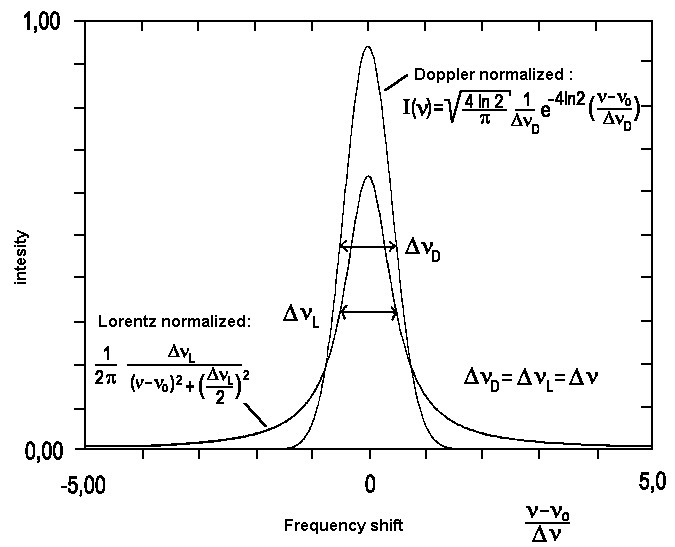
\includegraphics[width=(0.99\textwidth),height=(\textheight),keepaspectratio]{GLprofile}
\caption{Lorentzian vs Gaussian profile (in G manca un quadro all'esponente?!).}
\end{figure}


\end{usefull}

\clearpage

\subsubsection{Natural broadening (radiation damping)}

The motion of optical electron in a EM field of plane wave obey the (forced, damped) oscillation motion
\begin{equation*}
\ddot{x}+\gamma\dot{x}+\omega_0^2x=\frac{eE}{m}\cos{\omega t}
\end{equation*}

The oscillating (accelerating) charge radiate itself: the system losses energy.

Rate of energy radiation $P=\frac{2}{3}\frac{e^2\ddot{x}^2}{4\pi \epsilon_0c^3}$.

Classical absorption cross section
\begin{align*}
&a(\omega)=\frac{8\pi e^2}{3m_e^2c^4}[\frac{\omega^4}{(\omega^2-\omega_0^2)^2+\gamma^2\omega^2}]&\intertext{$\gamma$ is the classical damping constant}\\
&\gamma=(\frac{2e^2}{3m_ec^3})\omega_0^2
\end{align*}

Il principio di indeterminazione ci dice che un livello atomico non ha energia definita $E_i$ ma \'e una sovrapposizione di stati possibili attorno ad $E_i$: \mblock{\Delta \nu=\frac{\Delta E}{h}}. Transitions of electrons between levels doesn't correspond to specified energy difference.

Replace $\gamma$ with QM damping constant
\begin{align*}
&\Gamma_i=\sum_{l<i}A_{il}\\
&\Gamma_j=\sum_{l<j}A_{jl}
\end{align*}

\begin{definition}{Einstein coefficient $A_{ij}$}
The Einstein coefficient $A_{ij}$ is the probability in  unit of \si{\per\second} of a transition from upper level i to lower level j.
\end{definition}

The resulting profile for absorption cross section of a transition between two states reflects intrinsic energy width of both states: \mblock{\gamma_{nat}=\frac{\Delta E_i-\Delta E_f}{h/(2\pi)}}


\subsection{Absorption cross-section.}

Normalized absorption cross section for damping constant
\begin{align*}
&\phi_{\nu}=\frac{\frac{\Gamma}{4\pi^2}}{(\nu-\nu_0)^2+\frac{\Gamma^2}{(4\pi)^2}}\\
&\phi_{Max}=\phi_{\nu_0}=\frac{4}{\Gamma}\\
\end{align*}

For allowed transitions $\Delta\nu_{\frac{1}{2}}=\frac{\Gamma}{2\pi}\leq \SI{e-5}{\nano\meter}$ (FWHM), $\Delta\lambda=\frac{c}{\nu^2}\Delta\nu=\frac{2\pi}{3}\frac{e^2}{m_ec^2}\approx\SI{e-4}{\angstrom}$.

\subsection{Corpo nero}

L'energia irradiata per unit\'a di tempo per unit\'a di superficie nell'angolo solido $4\pi$ da un corpo nero di temperatura T
\begin{align*}
&(\int\,d\Omega I_{\nu}=)S_{\nu}=\frac{(4\pi)2 h\nu^3}{c^2}\frac{1}{\exp{\frac{h\nu}{KT}}-1}&\intu{nell'intervallo di frequenza $\nu,\nu+\,d\nu$, $\nu=\frac{c}{\lambda}$, $d\nu=-c\frac{d\lambda}{\lambda^2}$}\\
&(\int\,d\Omega I_{\lambda}=)S_{\lambda}=\frac{(4\pi)2 hc^2}{\lambda^5}\frac{1}{\exp{\frac{hc}{\lambda KT}}-1}&\intu{nell'intervallo di frequenza $\lambda,\lambda+\,d\lambda$}\\
&W=\sigma T^4&\intu{Legge di Stefan-Boltzmann}
\end{align*}

Il massimo di $S_{\lambda}$ segue la legge di Wien $\lambda_{Max}T=\const{}$.

\begin{definition}{Temperatura efficace}
\begin{equation*}
L=4\pi R^2\sigma T_e^4
\end{equation*}
\end{definition}

\begin{definition}{Temperatura di brillanza}
\begin{align*}
&I_{\nu}=B_{\nu}(T_b)\\
&L_{\lambda}=4\pi R^2\frac{2\pi hc^2}{\lambda^5}\frac{1}{\exp{\frac{hc}{\lambda KT_b}}-1}
\end{align*}
\end{definition}

Per il sole: $T_b(UV)\approx 5000\si{\kelvin}$, $T_b(V)\approx 6000\si{\kelvin}$

\begin{definition}{Temperatura di colore}
Temperature of a true blackbody is determined by intensity at two wavelength: match to shape of continous spectrum rather integrated power. 

\begin{equation*}
\frac{L_{\lambda_1}^O}{L_{\lambda_2}^O}=\frac{S_{\lambda_1}}{S_{\lambda_2}}
\end{equation*}

\end{definition}

\begin{definition}{Color index}
$B-V$ is defined by measurng luminisity with blue sensitive photographic plate (B) and with yellow-sensitive plate and yellow filter (V).
\end{definition}


\section{Righe dell'idrogeno.}

I livelli energetici dell'idrogeno sono \mblock{E_n=-\frac{\ER{}}{n^2},\ \ER{}\approx\SI{13.6}{\ev}}.

\begin{figure}[!ht]
\centering
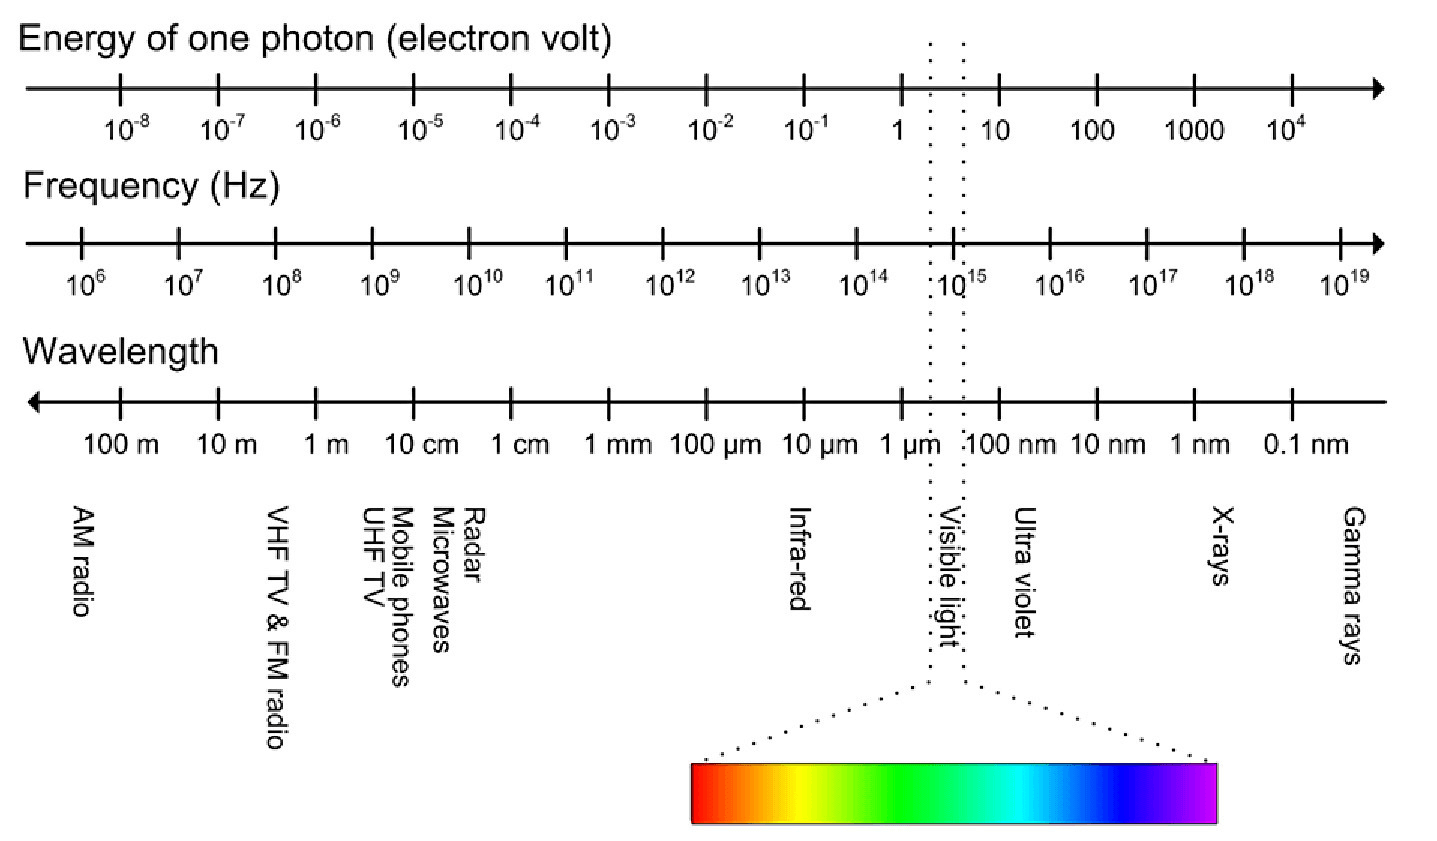
\includegraphics[width=(0.99\textwidth),height=(0.9\textheight),keepaspectratio]{PHevomega}
\caption{Spettro luminoso: energie, frequenze, regioni.}
\end{figure}

Le transizioni tra i livelli corrispondono a differenze di energie $E_{n,m}=\ER{}(\frac{1}{n^2}-\frac{1}{m^2})$
\begin{itemize}
    \item $n=1$: serie di Lyman (UV).
    \item $n=2$: serie di Balmer (V).
    \item $n=3$: serie di Paschen (IR).
\end{itemize}

\subsection{Popolazione dei livelli.}

A basse temperature H \'e neutro:
\begin{equation*}
    \frac{P(n)}{P(0)}\propto \exp{\frac{E_{0,n}}{KT}}
\end{equation*}
il rapporto \'e molto piccolo anche per $n=2$, primo eccitato.

A temperature intermedie (\SI{9520}{\kelvin}) la popolazione del primo eccitato $n=2$ raggiunge un massimo (stelle tipo spettrale A): le righe dell'idrogeno dominano lo spettro visibile.

\begin{figure}[!ht]
\centering
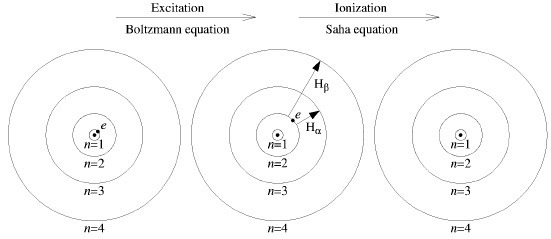
\includegraphics[width=(0.99\textwidth),height=(0.9\textheight),keepaspectratio]{boltzmansaha}
\caption{Determinazione popolazione livelli eccitati stati ionizzazione di H.}
\end{figure}

\begin{figure}[!ht]
\centering
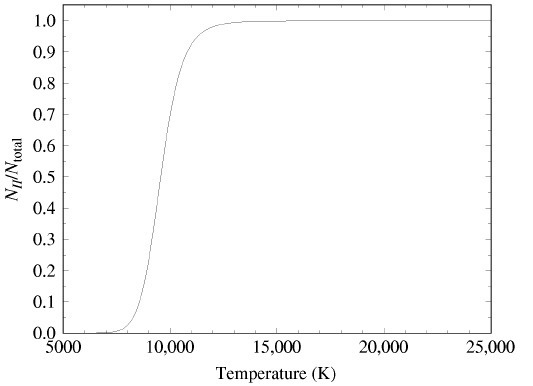
\includegraphics[width=(0.99\textwidth),height=(0.9\textheight),keepaspectratio]{HIIT}
\caption{Popolazione di HII.}
\end{figure}

\begin{figure}[!ht]
\centering
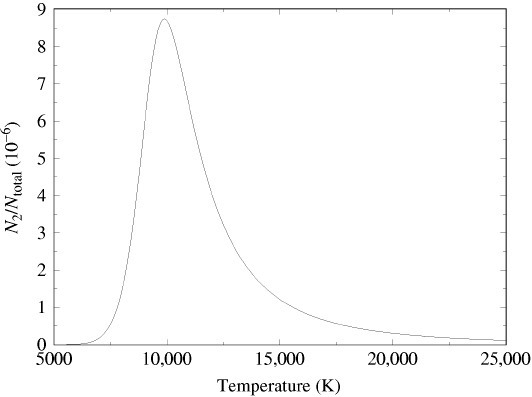
\includegraphics[width=(0.99\textwidth),height=(0.9\textheight),keepaspectratio]{HIn2pop}
\caption{Popolazione del livello primo eccitato di HI.}
\end{figure}

\clearpage

\section{Allargamento delle righe spettrali.}

\subsection{Allargamento (thermal) Doppler (GP)}

Lungo la linea di vista gli atomi hanno una distribuzione di velocit\'a gaussiana (moti termici e turbolenti)
\begin{align*}
&dn(v_e)\propto\exp{-\frac{v_e^2}{\alpha}}\,dv_e\\
&\alpha=\frac{2KT}{m}+v_{turb}^2
\end{align*}

La riga corrisponde ad una lunghezza d'onda diversa con
\begin{equation*}
\Delta\lambda\approx\frac{v_e}{c}\lambda
\end{equation*}

Per l'insieme degli atomi avremo una distribuzione di frequenze proprie

\begin{equation*}
\sigma(\nu)\propto\int\,d\nu*\exp{-A(\nu*-\nu_0)^2}\frac{1}{(\nu-\nu*)^2+(\frac{\gamma}{4\pi})^2}
\end{equation*}

Il profilo della riga \'e caratterizzato dalla curva pi\'u larga: Lorenziana, parametrizzata dalla larhezza naturale o gaussiana dalla distribuzione di velocit\'a.

Fatti:
\begin{itemize}
    \item Per il sole la gaussiana \'e pi\'u larga della lorenziana di un fattore \num{e3}.
\end{itemize}


\subsection{Allargamento da pressione (LP)}

La vicinanza di altre particelle perturba i livelli atomici (atmosfere con alta pressione): la condizione di equilibrio idrostatico in termini di profondit\'a ottica $\TDy{\tau}{P}=\frac{g}{\kappa}$ dice che nella regione $\tau\approx1$ la pressione $P_{Atm}\approx\frac{g}{\kappa}$, dove g \'e l'accelerazione di gravit\'a che determina l'allargamento da pressione mentre l'opacit\'a $\kappa$ varia meno rispetto a g.

Fatti:
\begin{itemize}
    \item La dominanza dell'allargamento da pressione nelle stelle di sequenza (nane) permette la classificazione empirica in classi di luminosit\'a.
\end{itemize}


\subsection{Allargamento quasi-statico.}

Effetto del campo esterno sull'atomo: perturba i livelli e cambia le energie di transizione. Distribuzione statistica nello spazio-tempo: distribuzione delle energie.

\mblock{\Delta t_{int}>\Delta T_{em}\approx\SI{e-9}{\second}}: nearby particles shift energy levels of emitting particle.

La larghezza \'e funzione soprattutto di $\rho$ (meno di $T$): si ha una dipendenza del tipo \mblock{\gamma\propto\exv{r}\expy{-n}}, con
\begin{itemize}
    \item Stark effect (WD): $n=3$.
    \item Van der Waals force (cool stars): $n=6$.
    \item Dipolar coupling between particles of same species: $n=3$.
\end{itemize}

\subsection{Allargamento da impatto (LP)}

Da un punto di vista semi-classico durante una collisione si interrompe l'assorbimento alla frequenza di transizione dell'atomo.

\mblock{\Delta t_{col}<\Delta T_{em}\approx\SI{e-9}{\second}}, funzione di $(T,\rho)$

\subsection{Allargamento dovuto alla rotazione.}

Ho un effetto Doppler di segno opposto nell zone simmetriche rispetto all'asse della superficie
\begin{equation*}
    \frac{\Delta\lambda}{\lambda}\approx\frac{\Delta v}{c}\approx2\frac{\omega R}{c}
\end{equation*}

Fatti:
\begin{itemize}
    \item Stelle rapidamente rotanti (A,O,B).
    \mblock{\omega R\approx v_F=\sqrt{\frac{2GM}{R}}\approx\SI{e3}{\kilo\meter\per\second}} e \mblock{\frac{\Delta\lambda}{\lambda}\approx\num{e-3}}: nel visibile $\Delta\lambda\approx\SI{10}{\angstrom}$.
    \item Le classi O,B sono rotatori veloci, il tipo A comprende rotatori lenti e veloci e $Ap$, i tipi spettrali pi\'u freddi da F in poi sono rotatori lenti.
\end{itemize}


\section{Astro-spettroscopia.}

\subsubsection{Spectral resolution.}

A varie dispersioni sul ricevitore gli spettri ci danno informazioni diversi
\begin{itemize}
    \item Bassa dispersione: \SI{e2}{\angstrom\per\milli\meter}.
    
    Tipo spettrale.
    
    \item Media dispersione: \numrange{10}{100}\si{\angstrom\per\milli\meter}.
        
    Velocit\'a radiale, allargamento righe: P,T, righe peculiari.
        
    \item Alta dispersione: $\leq$\SI{10}{\angstrom\per\milli\meter}.
    
    $W_{\lambda}(\eta_{\lambda})$: analisi quantitativa,  ricostruzione dell'atmosfera.

\end{itemize}


\subsubsection{Moto radiale.}

Le righe sono spostate verso il rosso/blu
\begin{align*}
    &\frac{\Delta\lambda}{\lambda}=z\approx\frac{v}{c}&\intu{small $v$}\\
    &1+z=\gamma(1+\frac{v_{\parallel}}{c})\\
    &v_{los}=c\exv{\frac{\Delta\lambda}{\lambda}}_{Righe}
\end{align*}

Classi di osservazioni:
\begin{itemize}
    \item Binarie spettroscopiche
    \item Stelle pulsanti
    \item Legge di Hubble: $v_{rad}\approx c$
\end{itemize}

\subsection{Gravitational red-shift}

Per oggetti densi \'e osservabile uno spastamento Doppler delle righe di assorbimento dovuto alla differenza tra energia gravitazionale sulla superficie della stella ed energia al punto d'osservazione:
\begin{align*}
&V_{grav}=\frac{GM}{Rc}\\
&\frac{\Delta\lambda}{\lambda}=\frac{E}{\Delta E}\overset{?}{=}\frac{Rc^2}{GM}
\end{align*}

\section{Classificazione degli spettri stellari}

In un grafico $U-B$ vs $B-V$ una successione di corpi neri di temperatura variabile \'e approssimativamente una linea retta.

\begin{figure}[!ht]
\centering
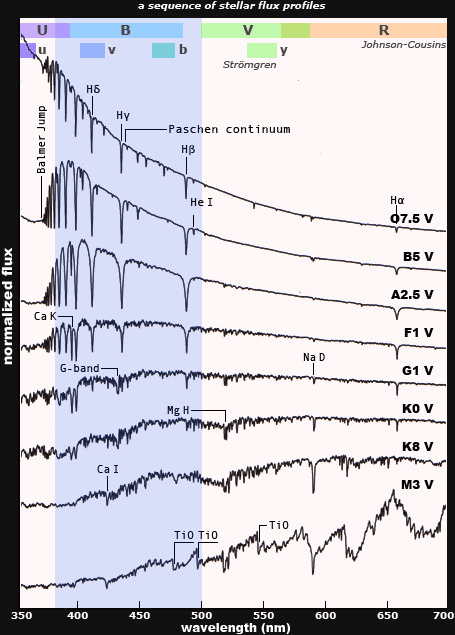
\includegraphics[width=(0.99\textwidth),height=0.9\textheight,keepaspectratio]{sequenceFP}
\caption{Sequence stellar flux profile.}
\end{figure}

La classificazione stellare consiste di una lettera per il tipo, numero per il sottotipo e un numero romano per la classe di luminosit\'a (I supergiganti, III giganti, IV subgiganti, V nane). Il tipo spettrale \'e individuato dalla distribuzione del continuo e dalla presenza di alcune righe.

La classe di luminosit\'a \'e individuata dalle caratteristiche delle righe: Larghezza/pressione supericiale.

\begin{figure}[!ht]
\centering
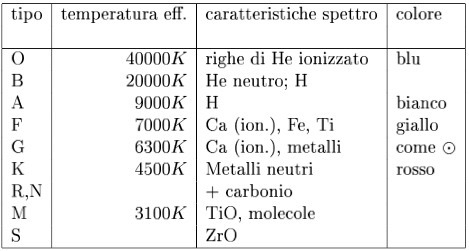
\includegraphics[width=(0.8\textwidth),height=(\textheight-11mm),keepaspectratio]{types}
\caption{Star types.}
\end{figure}

Fatti:
\begin{itemize}
\item O stars (\SI{30000}{\kelvin}): hottest stars, continuum strong in UV.

Strong He II lines in absorption, sometimes with few lines; He II dominates emission; He I lines weak but increasing in strength
from O5 to O9; hydrogen Balmer lines prominent but
weak relative to later types; lines of Si IV, O III, NIII
and C IV.

\item B stars (\SI{20000}{\kelvin}).

He I lines dominate, with maximum strength at B2; He I dominates He II lines virtually absent; hydrogen lines strengthening
from B0 to B9; Mg II and Si II lines

\item A stars (\SI{10000}{\kelvin}). 

Hydrogen lines reach maximum strength at A0; hydrogen Balmer lines dominate of ionised metals (Fe II, Si II, Mg II) at maximum strength near A5; Ca II lines strengthening; lines of neutral
metals appearing weakly.

\item F stars (\SI{7000}{\kelvin}).

Hydrogen lines weakening rapidly while H and K lines of CaII strengthen; neutral metal (Fe I and Cr I) lines gaining on ionised metal lines by large F

\item G stars (\SI{6000}{\kelvin}).

Hydrogen lines very weak; Ca II H and K lines reach maximum strength near G2; neutral metal (Fe I, Mn I,Ca I) lines strengthening while ionised metal lines
diminish; molecular G band of CH becomes strong.

\item Il sole \'e una stella di tipo G2.

\item K stars (\SI{4000}{\kelvin}).

Hydrogen lines almost gone; Ca lines strong; neutral metal lines very prominent; molecular bands of TiO begin (K2)
to appear by late K.

\item M stars (\SI{3000}{\kelvin}).

Neutral metal lines very strong; molecular bands prominent with TiO bands dominating by M5; vanadium oxide bands appear.

\end{itemize}


\begin{figure}[!ht]
\centering
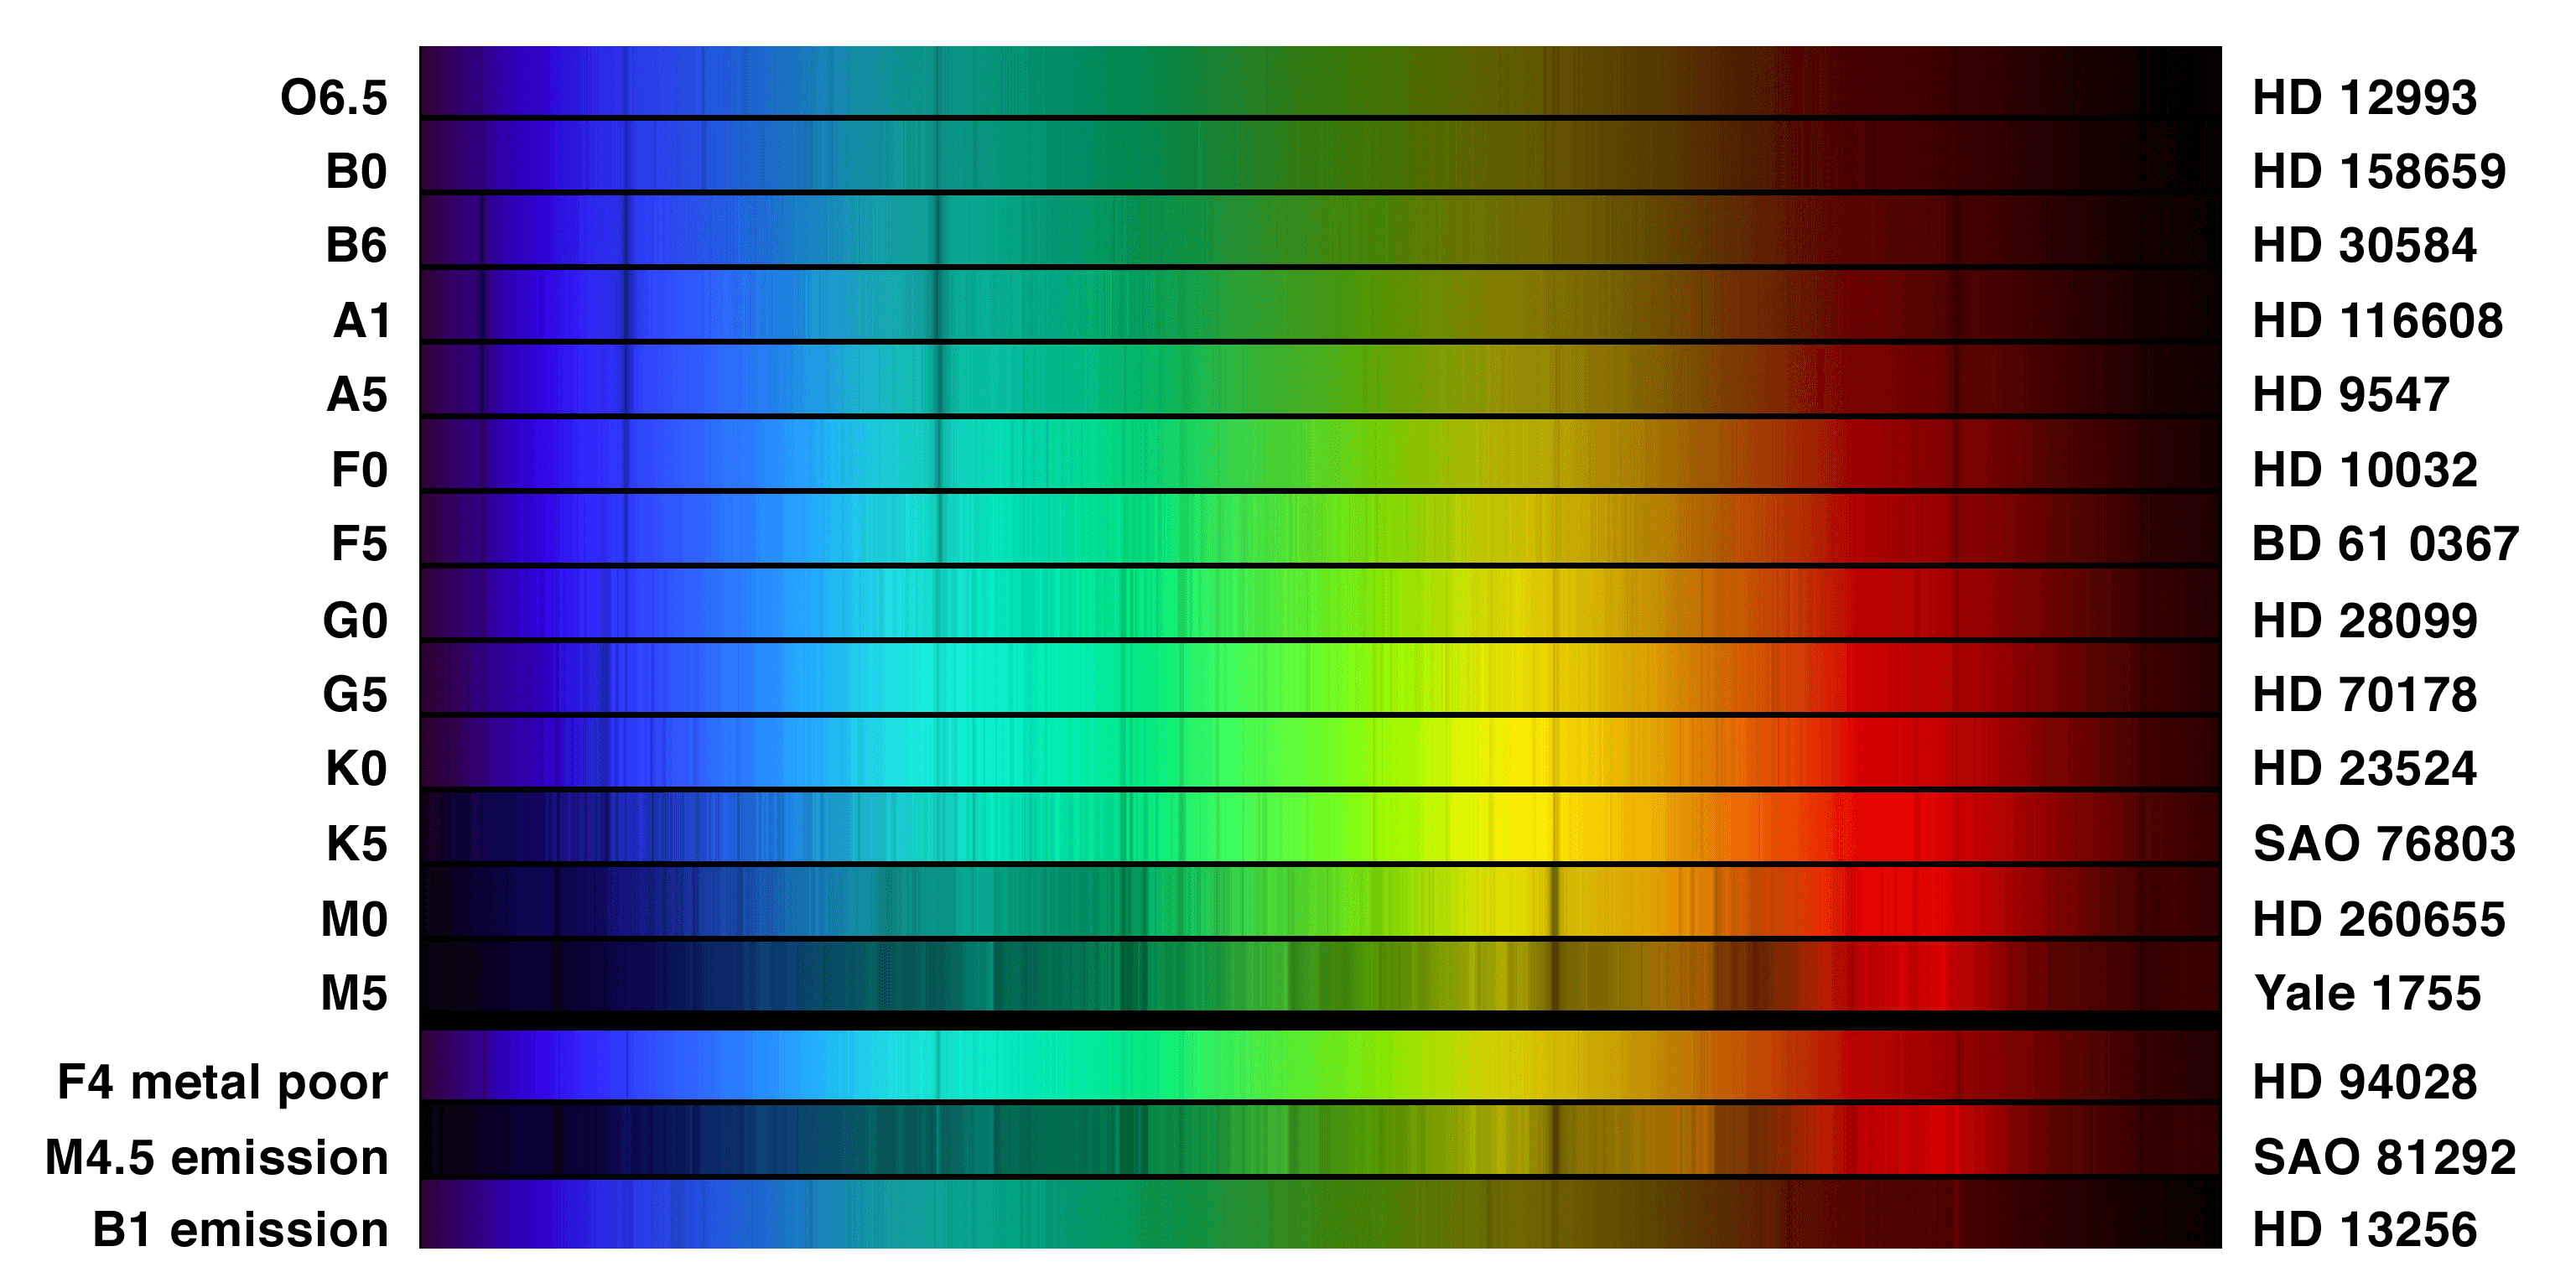
\includegraphics[width=(0.99\textwidth),height=\textheight,keepaspectratio]{spectral}
\caption{Spectral types.}
\end{figure}

\begin{figure}[!ht]
\centering
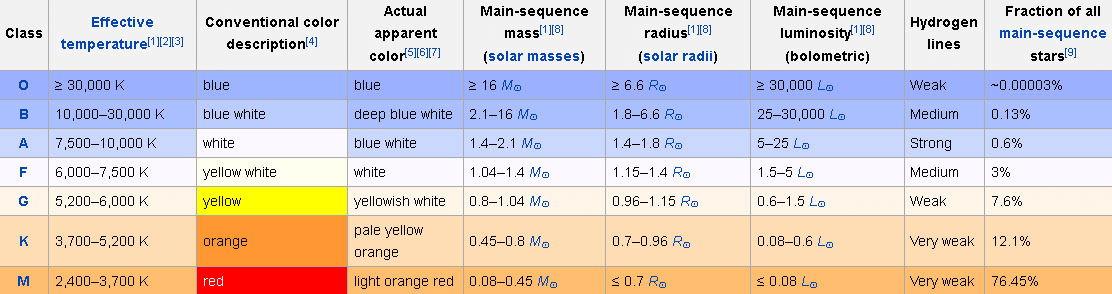
\includegraphics[width=(\textwidth),height=(\textheight-11mm),keepaspectratio]{classprop}
\caption{Classi stellari.}
\end{figure}

\clearpage



\chapter{Relazioni massa/luminosit\'a. Diagramma di \hr{}.}
\PartialToc

\subsection{Massa-Luminosit\'a}

\begin{usefull}{Massa-Luminosit\'a (relazione).}
\begin{align*}
    &\frac{L}{\lsun{}}\approx0.23(\frac{M}{\msun{}})\expy{2.3},\ (M<0.43\msun{})\\
    &\frac{L}{\lsun{}}\approx(\frac{M}{\msun{}})^4,\ (0.43\msun{}<M<2\msun{})\\
    &\frac{L}{\lsun{}}\approx1.5(\frac{M}{\msun{}})\expy{3.5},\ (2\msun<m<20\msun{})\\
    &\frac{L}{\lsun{}}\approx3200\frac{M}{\msun{}},\ (m>20\msun{})
\end{align*}
\end{usefull}



\section{Importanti relazioni semi-empiriche.}

\subsection{Massa-Luminosit\'a}

\begin{equation*}
    (\frac{L}{\lsun{}})=(\frac{M}{\msun{}})\expy{\frac{1}{4}}
\end{equation*}

\begin{todo}{Importanti relazioni semi-empiriche.}
clay pg 470-472.
$\S 1.6$ stellar interior
\end{todo}

\section{Diagrammi di HR: magnitudine vs colore.}


Considero il diagramma $M_V$ vs $(B-V)$ o $M_{B}$ vs spectral type (per stelle vicine) (\mblock{M_B=-2.5\log{\frac{L}{\lsun{}}}+4.72})

\subsection{Diagramma di HR per stelle vicine.}

\begin{figure}[!ht]
\centering
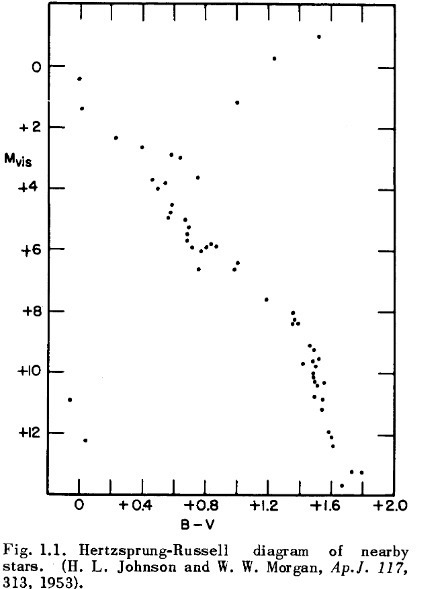
\includegraphics[width=(\textwidth),height=(0.8\textheight),keepaspectratio]{nearbyHR}
\caption{Diagramma HR di stelle vicine.}
\end{figure}

\clearpage

\subsection{Diagramma di HR per associazioni di stelle.}

Considero il diagramma di HR per associazioni fisiche di stelle.


La struttura di una stella \'e univocamente definita da massa, composizione chimica iniziale ed et\'a: un diagramma di ammasso si pu\'o vedere come una sequenza di stelle con massa variabile e stessa composizione iniziale ed et\'a.

\begin{figure}[!ht]
\centering
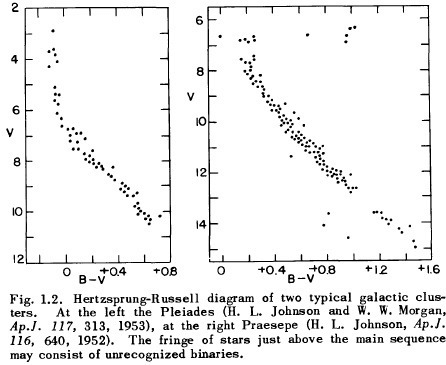
\includegraphics[width=(\textwidth),height=(\textheight-11mm),keepaspectratio]{GCHR}
\caption{Diagramma di HR di un cluster.}
\end{figure}


\begin{figure}[!ht]
\centering
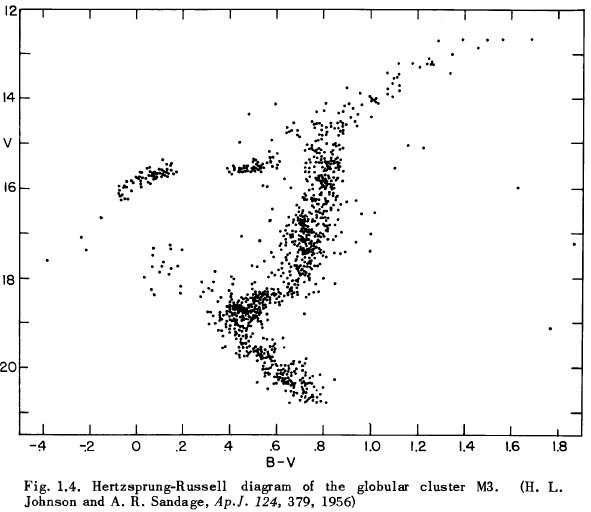
\includegraphics[width=(\textwidth),height=(\textheight-11mm),keepaspectratio]{GlobularCHR}
\caption{Diagramma di HR di un ammasso globulare.}
\end{figure}

\clearpage

\subsection{Evolution of a cluster of stars.}

\subsubsection{Evolution from main sequence.}

Il processo di fusione $4H\to He$ produce \SI{6.4e18}{\erg\per\gram}.

Suppongo che una stella di massa M si allontani dalla sequenza principale quando ha costituito un core di He di massa $fM$:

se $X_H$ \'e la frazione di H in massa originaria si deve convertire in He una massa $fX_HM$ di H quindi l'energia irradiata \'e $E=fX_HM(\num{6.4e18})=\num{1.3e52}fX_H\frac{M}{\msun{}}\si{\erg}$.

La vita di sequenza principale pu\'o essere stimata
\begin{equation*}
    \tau_E=\frac{E}{L}=\num{1.1e11}fX_H\frac{M/\msun{}}{L/\lsun{}}\si{\year}
\end{equation*}

Fatti:
\begin{itemize}
    \item Per stella solar-like $f=15\%$: using M/L relatioship
    \begin{equation*}
    \tau_E=\num{12e9}(\frac{L}{\lsun{}})\expy{-\frac{3}{4}}\si{\year}
    \end{equation*}
    \item Posso approssimare l'et\'a di un ammasso con l'et\'a delle sue stelle pi\'u luminose. 
\end{itemize}

Ad alta luminosit\'a la linea della sequenza principale svolta a destra.

\subsubsection{Turn-off: ramo delle giganti.}

Una classificazione dei diagrammi in sequenze di $(B-V)_{\text{Turn-off}}$ crescenti corrisponde ad una sequenza di et\'a: turn-off blue per ammasso giovane, turn-off giallo ammasso vecchio.


\begin{figure}[!ht]
\centering
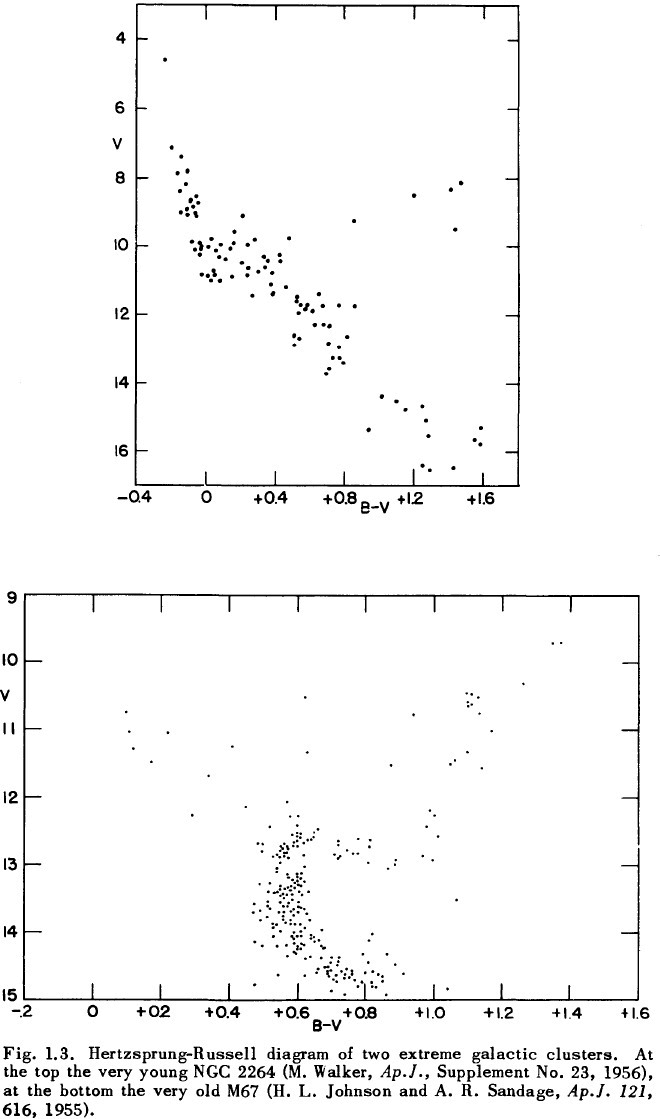
\includegraphics[width=(\textwidth),height=(0.9\textheight),keepaspectratio]{extremeGCHR}
\caption{Diagramma di HR di cluster giovane (in alto) vecchio (in basso).}
\end{figure}

\clearpage

\section{Caratteristiche delle stelle nelle zone del diagramma di HR.}

\begin{figure}[!ht]
\centering
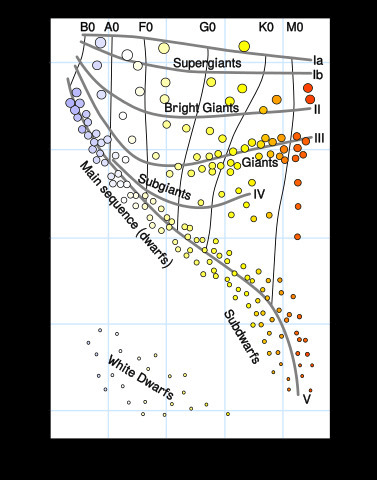
\includegraphics[width=(\textwidth),height=(0.9\textheight),keepaspectratio]{HRpizza}
\caption{Diagramma di HR: MS, WD, SD, giant branch.}
\end{figure}

\subsection{Passaggio al diagramma raggio-Luminosit\'a.}

Passo alla rappresentazione con in ordinata L e in ascissa $T_e$:

\begin{align*}
    &\log{\frac{L}{\lsun{}}}=\frac{1}{2.5}(M_{B\odot}-M_B)\\
    &=4\log{\frac{T_e}{T_{e\odot}}}+2\log{\frac{R}{\rsun}}
\end{align*}

\begin{figure}[!ht]
\centering
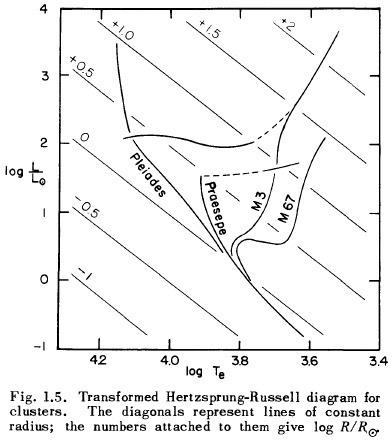
\includegraphics[width=(\textwidth),height=(\textheight-11mm),keepaspectratio]{CsHR}
\caption{Diagramma HR $L$ vs $T_e$.}
\end{figure}

\clearpage

\subsection{Nane.}



\subsection{Sub-nane.}

Caratteristiche:
\begin{itemize}
    \item Deboli righe di assorbimento.
    \item Parallela alla MS circa 1 magnitudine superiore.
    \item Per pari $T_e$ $\log{\frac{L_{SN}}{L_{MS}}}=-0.4$.
\end{itemize}

Le differenze di luminosit\'a e di caratteristiche spettrali sono attribuibili alla diversa composizione chimica.

Fatti:
\begin{itemize}
    \item La sequenza principale degli ammassi globulari coincide con quella delle sub-nane.
\end{itemize}

\subsection{Nane bianche.}

Caratteristiche:
\begin{itemize}
    \item Alta densit\'a superficiale: righe allargate.
    \item Raggio quasi costante circa $\frac{1}{100}\rsun{}$.
    \item Oggetti estremamente densi.
    \item Fase finale evoluzione stellare.
\end{itemize}


\section{Popolazioni stellari.}

Fatti:
\begin{itemize}
\item Existence in late F early G stars of strong-line and weak-line with different kinematical properties: generally the strong lines have low velocity, the weak line higher velocity.
\end{itemize}

\begin{figure}[!ht]
\centering
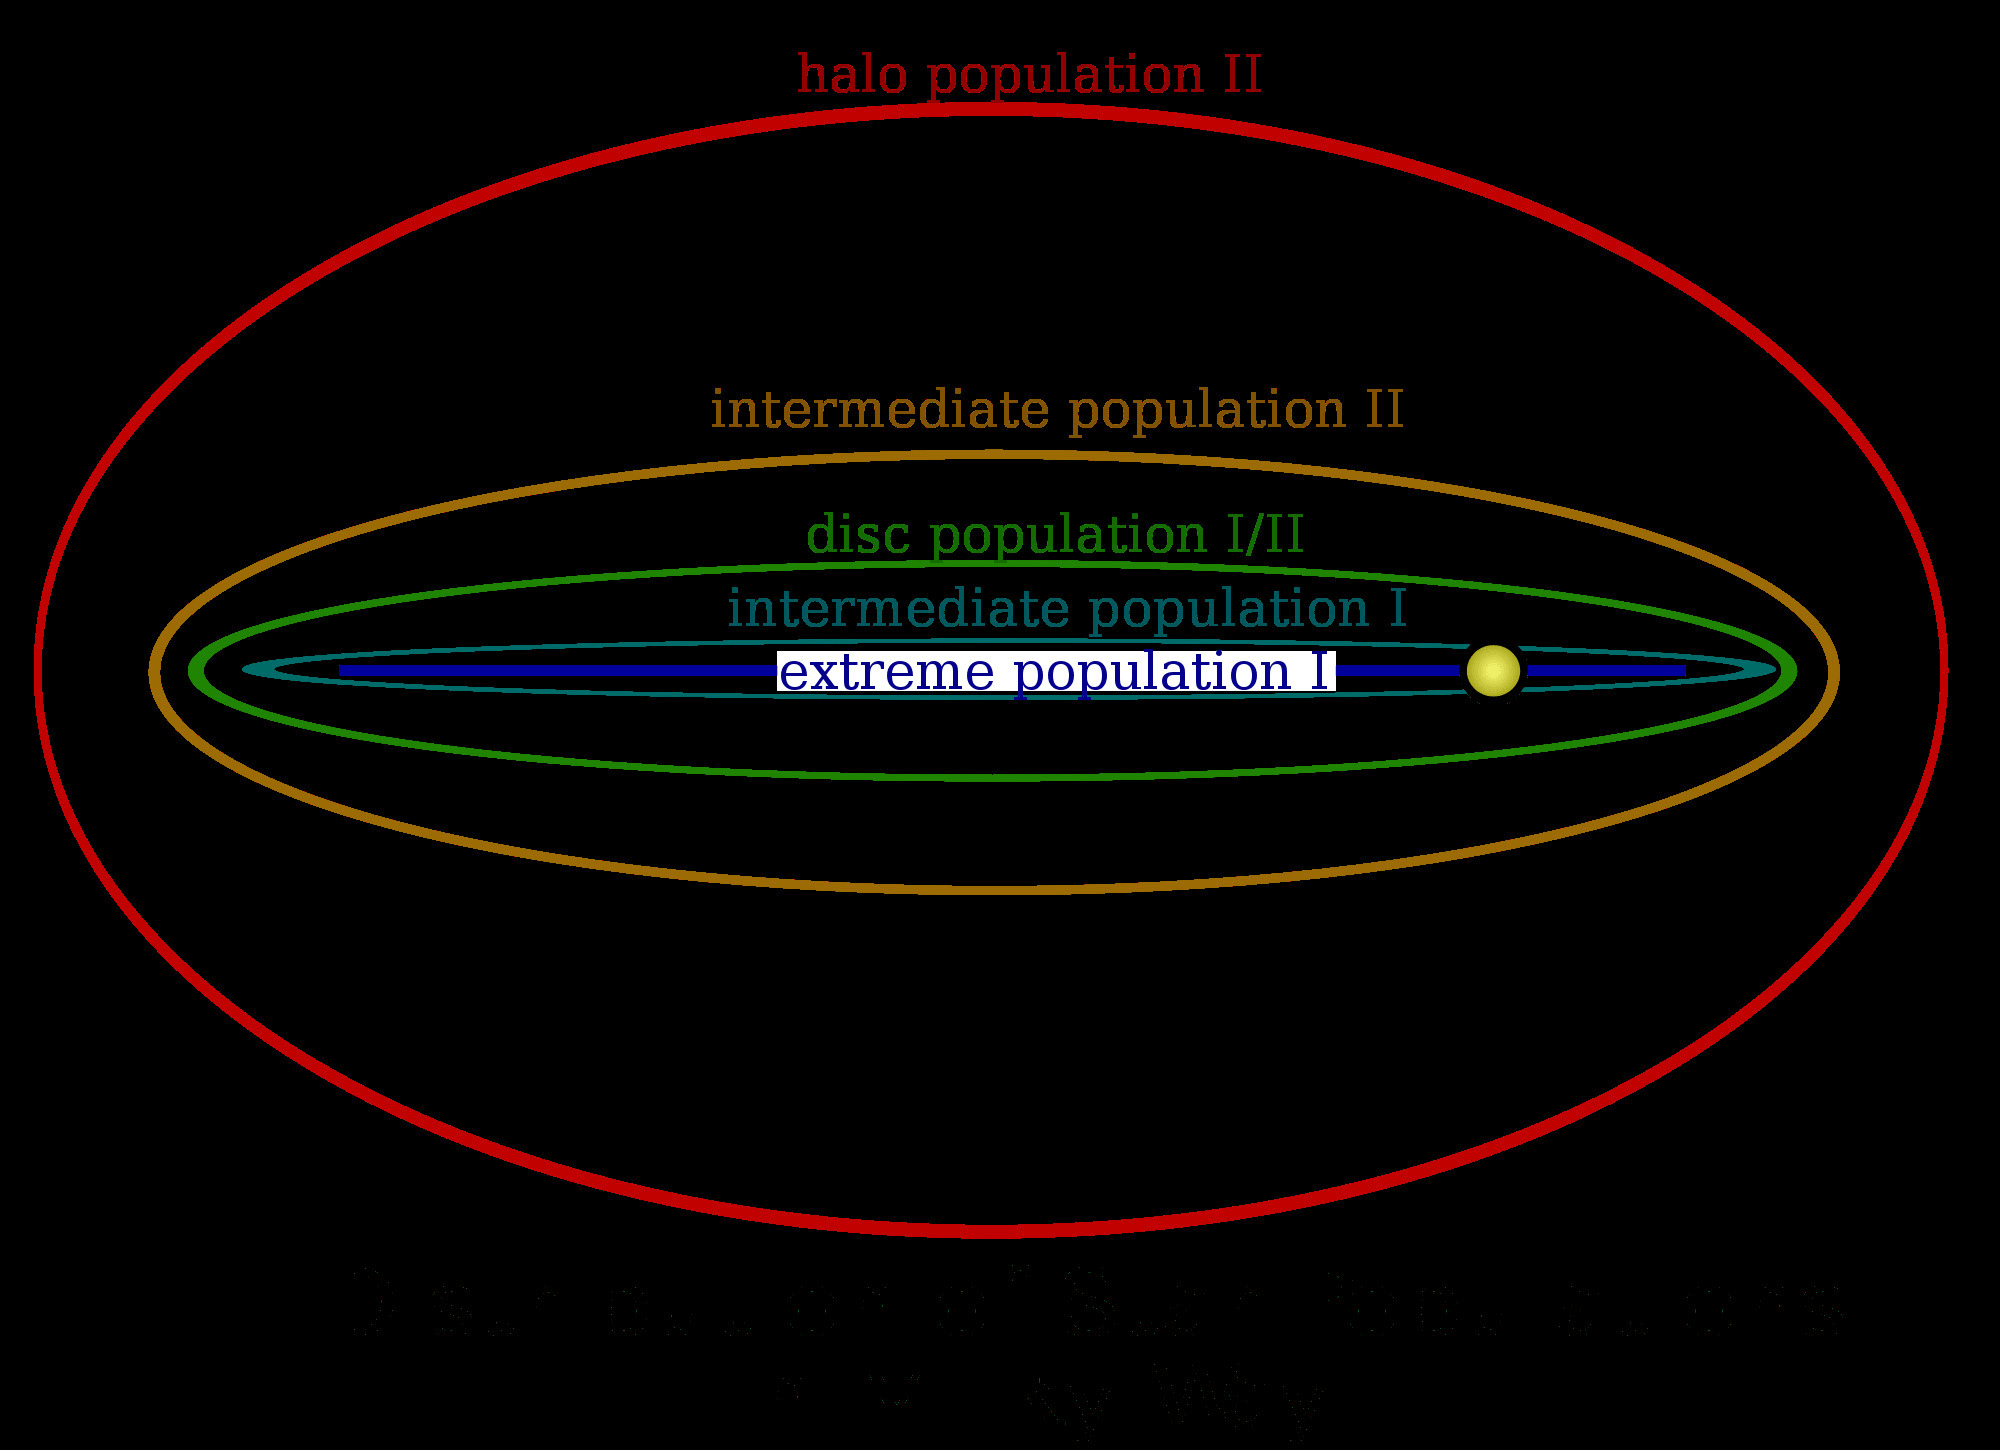
\includegraphics[width=(\textwidth),height=(\textheight-11mm),keepaspectratio]{Starpop}
\caption{Popolazioni stellari: distribuzione galattica.}
\end{figure}

\begin{figure}[!ht]
\centering
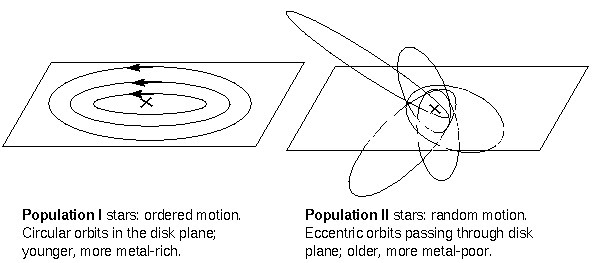
\includegraphics[width=(\textwidth),height=(\textheight-11mm),keepaspectratio]{starpops}
\caption{Popolazioni stellari: differenze orbitali.}
\end{figure}

\subsection{Cluster di stelle.}

\begin{definition}{Star cluster.}
Is a group of stars that have a much stronger gravitational attraction to each others than to general field of stars.
\end{definition}

\subsubsection{Globular cluster.}



\begin{itemize}
    \item Number of stars: approx. \num{e5}.
    \item Far from the Sun: magnitude of RR Lyra stars.
    \item Location: Corona or galactic nucleus.
    \item Diameter of high density region approx \SI{10}{\parsec}, density \SI{e3}{\per\parsec}.
    \item Diameter \numrange{50}{100} \si{\parsec}.
    \item Color of the brightest: red.
    \item Densit\'a di stelle (\si{\cubic\parsec}): \numrange{0.5}{e3}.
    \item Nomi: M3
\end{itemize}

\subsubsection{ Open Cluster (Galactic cluster).}

\begin{itemize}
    \item Few-thousands stars randomly distributed.
    \item Found in galactic disc.
    \item Location: disk.
    \item Number of stars: \numrange{50}{e3}.
    \item Color of the brightest: red/blue.
      \item Densit\'a di stelle (\si{\cubic\parsec}): \numrange{0.1}{10}.
    \item Nomi: Hyades, Pleiades.
\end{itemize}

\subsubsection{Association.}

Open cluster containing most luminous main sequence stars of type $O/B$. O stars are not randomly distributed: O/B/WR are scattered in a region of \SI{100}{\parsec}.

\begin{itemize}
    \item Location: spiral harms.
    \item Diameter: \numrange{30}{200}\si{\parsec}
    \item Number of stars \numrange{10}{100}?
    \item Color of the brightest: blue.
      \item Densit\'a di stelle (\si{\cubic\parsec}): \num{0.01}.
    \item Nomi: Orion.
\end{itemize}
    


Fatti:
\begin{itemize}
    \item Le supergiganti blu sono stelle giovani vicine a nubi interstellari.
    \item Espansione di ammassi/associazioni contenenti SG blue permette, ricostruendo all'indietro il loro moto, di limitare superiormente la loro et\'a a \SI{e8}{\year}.
    \item Le galassie ellittiche e gli ammassi globulari appaiono prive di gas interstellare e polvere (Highly stable dynamical system).
\end{itemize}


\subsection{Comportamento cinematico}

\'E possibile separare le stelle vicine in due gruppi:
\begin{itemize}
    \item Alta velocit\'a sul piano galattico.
    
    Giganti rosse (HR simile agli ammassi globulari), subnane, 
    
    \item Bassa velocit\'a sul piano galattico.
    
    Stelle di tipo O/B (HR simile ad ammassi galattici), nubi interstellari.
\end{itemize}

Fatti:
\begin{itemize}
    \item Gli ammassi galattici presentano moto d'insieme di moderata velocit\'a a differenza degli ammassi globulari.
    \item Ad alta velocit\'a sul piano galattico corrisponde alta velocit\'a ortogonale: configurazione sempre pi\'u sferica.
    \item Le stelle ad alta veloci\'a hanno un moto retrogrado sul piano galattico (alone esterno).
\end{itemize}

\subsection{Evoluzione della galassia.}

Trasformazione di una struttura quasi-sferica ad un disco accompagnato da un rarefatto alone.

\begin{todo}{High/low velocity galactic plane}
Moto retrogrado
\end{todo}


\subsubsection{Popolazione I.}

Si distinguono spettroscopicamente stelle con righe forti (lente) e stelle con righe deboli (veloci).

\begin{itemize}
    \item (Young) extreme pop I.
    
    Typical member: Blue giant, variabili T Tauri, Cefeidi.
    
    Where: ammassi aperti, galactic cluster, braccia a spirale, G (spirale, irregolare).
    
    AVG velocity: \SI{8}{\kilo\meter\per\second}. Shape of subsystem: flat. Distanza dal PG: \SI{60}{\parsec}.
    
    Metallicit\'a: $\frac{Z}{Z_{\odot}}>1$.
    
    Et\'a (risp. universo): \numrange{0}{0.005}.
    
    \item (Int.) Pop I. 
    
    Typical member: Stelle a forti righe metalliche, Supernovae II, vicine del Sole.
    
    AVG velocity: \SI{10}{\kilo\meter\per\second}.
    
    Distanza dal piano galattico: \SI{160}{\parsec}.
    
    Metallicit\'a: $\frac{Z}{Z_{\odot}}>0.75$.
    
    Et\'a (risp. universo): \numrange{0.05}{0.25}.
    
    Where: Disco.
    
    \item (Old/disc) Pop I. 
    
    Typical member: Stelle a deboli righe metalliche, novae,nebulase planetarie, RR Lyrae, Periodic ($P<0^d.4$).
    
    AVG velocity: \SI{16}{\kilo\meter\per\second}. Distanza dal piano galattico: \SI{300}{\parsec}.
    
    Metallicit\'a: $\frac{Z}{Z_{\odot}}>0.5$.
    
    Et\'a (risp. universo): \numrange{0.25}{0.8}.
    
    Where: Disco, nucleo galattico (Bulges).

\end{itemize}

\subsubsection{Popolazione II.}

Si distinguono ammassi globulari e stelle ad alta velocit\'a.

\begin{itemize}
    \item Intermediate Pop. II:
    
    Stelle: Stelle ad alta velocit\'a, variabili a lungo periodo, RR Lyrae.
    
    AVG velocity(ortogonale al piano galattico): \SI{25}{\kilo\meter\per\second}.
    
    Where: Galassie ellittiche, disco spesso, ammasso globulare.
    
    Distanza dal piano galattico: \SI{500}{\parsec}.
    
    Metallicit\'a: $\frac{Z}{Z_{\odot}}=0.25$.

    Et\'a in et\'a dell'universo: \numrange{0.8}{1}.

    \item Pop II di Bulge:
    
    Where: Nucleo galattico.
    
    Stelle: Nebulose planetarie, Cefeidi.
    
    Metallicit\'a: $\frac{Z}{Z_{\odot}}=\numrange{0.1}{2.}$.
    
    Et\'a in et\'a dell'universo: \numrange{0.5}{1}.
    
    \item Extreme (halo) Pop. II:
    
    Stelle: Bright red giants, globular cluster, subdwarf, RR Lyrae $\Pi>0^d.4$, ramo orizzontale HR.
    
    AVG velocity(ortogonale al piano galattico): \SI{75}{\kilo\meter\per\second}.
    
    Where: Ammassi globulari, galassie ellittiche.
    
    Distanza dal piano galattico: \SI{2000}{\parsec}.
    
    Metallicit\'a: $\frac{Z}{Z_{\odot}}=\numrange{0.03}{0.1}$.

    Et\'a in et\'a dell'universo: \numrange{0.9}{1}.

    \item Pop II di Bulge:
    
    Where: Nucleo galattico.
    
    Stelle: Nebulose planetarie, Cefeidi.
    
    Metallicit\'a: $\frac{Z}{Z_{\odot}}=\numrange{0.1}{2.}$.
    
    Et\'a in et\'a dell'universo: \numrange{0.5}{1}.
\end{itemize}



